\documentclass[letterpaper]{article}

% AAAI 2027 anonymous submission style
\usepackage[submission]{aaai2027}

% Required packages
\usepackage[hyphens]{url}
\usepackage{graphicx}
\urlstyle{rm}
\def\UrlFont{\rm}
\usepackage{natbib}
\usepackage{caption}
\frenchspacing

% Mathematical formulas
\usepackage{amsmath}
\usepackage{amssymb}

% Professional tables
\usepackage{booktabs}
\usepackage{multirow}

% Required PDF metadata
\pdfinfo{
/TemplateVersion (2027.1)
}

% Number sections and subsections.
% Subsubsections remain unnumbered.
\setcounter{secnumdepth}{2}

% Paper title
\title{Diffusion-Driven Graph Reconstruction and Cross-View Contrastive Learning for Bundle Recommendation}

% Anonymous author information
\author{
Anonymous Submission
}

\affiliations{
}

\begin{document}

\maketitle


\begin{abstract}
Bundle recommendation integrates bundle-level feedback and item-level information to model users' preferences for sets of items. Recent research has integrated user-bundle (U-B) interactions, user-item behavior, and bundle composition into a common multi-view framework that combines graph-based modeling, representation fusion, and contrastive learning. Despite this progress, two challenges remain: (1) noisy U-B interactions can spread misleading signals through graph propagation; (2) sparse U-B feedback limits preference learning for users with few bundle interactions. To address these challenges, we propose ReCoBR, a framework that combines diffusion-driven graph reconstruction with cross-view contrastive learning. ReCoBR pretrains user and bundle embeddings, learns a user-conditioned latent diffusion model to refine aggregated historical bundle representations, and uses the refined preferences to re-score observed interactions and reconstruct the U-B graph. To adapt the denoising process to bundle recommendation, we introduce a bundle-set consistency loss that complements preference reconstruction by encouraging agreement between the refined preference and historical bundle embeddings. The reconstructed U-B view then anchors cross-view contrastive learning before representation fusion. User-side and bundle-side objectives connect U-B representations with their user-item and bundle-item counterparts, allowing behavioral and compositional information to support preference learning under sparse U-B feedback. Experiments on three public benchmarks show that ReCoBR outperforms the compared baselines.
\end{abstract}


\section{Introduction}

Bundle recommendation (BR) aims to match users with collections of related items, such as music playlists and fashion outfits \cite{chen2019dam,ma2022crosscbr}. For platforms, BR can create additional sales opportunities; for users, it can simplify the discovery and selection of collections suited to their needs \cite{ma2022crosscbr,ma2024multicbr}. Learning the preferences underlying these recommendations involves modeling bundle-level choices through user-bundle (U-B) interactions and item-level behavior through user-item (U-I) interactions, with bundle-item (B-I) affiliations linking individual items to bundles. Effectively integrating information about user behavior and bundle composition is therefore key to accurately modeling users' preferences and providing personalized bundle recommendations.

Early approaches pursue this goal through joint learning at the bundle and item levels. DAM, for example, jointly models U-B and U-I interactions and uses attention to aggregate constituent-item representations into bundle representations \cite{chen2019dam}. Graph-based approaches further exploit the collaborative structure formed by these relations. BGCN uses graph propagation to model preferences at both the bundle and item levels, linking items to bundles through B-I affiliations \cite{chang2020bgcn}. This graph formulation captures higher-order collaborative information while retaining two perspectives on users' bundle preferences.

Learning separate views also raises the question of how they can inform one another. CrossCBR addresses this question through cross-view contrastive learning, encouraging agreement between the representations of the same user or bundle across the bundle and item views \cite{ma2022crosscbr}. MultiCBR extends the formulation to three views by encoding U-B interactions, U-I interactions, and B-I affiliations separately \cite{ma2024multicbr}. It combines these representations before prediction, allowing information from different views to interact in bundle scoring, and applies contrastive learning to the fused representation. DGMAE explores another form of cross-view cooperation by distilling first- and higher-order U-B knowledge into item-view representation learning \cite{ren2023dgmae}.

These advances demonstrate the benefits of coordinating complementary views, while also highlighting the central role of U-B interactions in bundle recommendation: U-B interactions define the bundle-view graph used for propagation, provide direct supervision for bundle ranking, and supply the bundle-level signal that is coordinated with auxiliary views in multi-view learning \cite{ma2022crosscbr,ma2024multicbr,ren2023dgmae}. However, existing multi-view methods mainly focus on representation construction and cross-view coordination, typically treating the observed U-B feedback itself as a given rather than explicitly examining or refining the information it provides. At the same time, the reliability and sufficiency of observed U-B feedback remain concerns, as it can be noisy and sparse. Based on the above analysis, we identify the following two challenges.

\textbf{Challenge 1: Noise in user-bundle interactions.} Implicit feedback may include interactions that do not faithfully reflect users' preferences \cite{wang2021adt,jiang2026cafu}. Once incorporated as edges in the U-B graph, such interactions can introduce misleading signals that spread through neighborhood aggregation into the representations used for bundle ranking \cite{wu2021sgl}. At the same time, observed U-B interactions contain useful bundle-level evidence about each user's preferences. The challenge is therefore to limit the influence of potentially misleading connections during graph propagation without discarding useful personalized evidence.

\textbf{Challenge 2: Sparse user-bundle feedback.} Even reliable U-B feedback provides limited direct evidence when a user has interacted with only a few bundles. U-I interactions and B-I affiliations can supplement this evidence by revealing the user's item-level interests and the composition of bundles. However, interest in an individual item does not necessarily imply preference for the complete bundle \cite{ren2023dgmae}. The challenge is therefore to use this auxiliary information to supplement sparse U-B feedback while retaining users' bundle-level choices as the reference for preference learning.

To address these challenges, we propose \textbf{ReCoBR} (Reconstruction and Contrastive Learning for Bundle Recommendation), which combines diffusion-driven U-B graph reconstruction with cross-view contrastive learning. ReCoBR first pretrains user and bundle embeddings on the U-B graph with LightGCN \cite{he2020lightgcn} and aggregates each user's historical bundle embeddings into a preference representation. Conditioned on the pretrained user embedding, a latent diffusion model learns to recover this representation from Gaussian perturbations \cite{wang2023diffrec,zhao2024ddrm}, while a bundle-set consistency loss encourages the recovered preference to align with the user's historical bundle embeddings. The denoiser then iteratively refines the preference representation and re-scores observed interactions, retaining each user's highest-scoring connections for graph propagation; the original U-B interactions continue to provide ranking supervision. Using the reconstructed U-B graph alongside the U-I and B-I relations, ReCoBR learns view-specific user and bundle representations. Before fusion, U-B--U-I and U-B--B-I contrastive objectives jointly optimize the paired representations on both the user and bundle sides, with the reconstructed U-B view as their common reference. These objectives allow behavioral and compositional evidence to support bundle-level preference learning under sparse U-B feedback.

Our main contributions are as follows:

\begin{itemize}
\item We develop a diffusion-driven U-B graph reconstruction framework that integrates pretraining, user-conditioned historical preference refinement, and observed-interaction selection, supplemented by a bundle-set consistency objective.
\item We introduce cross-view contrastive objectives that use the reconstructed U-B view as a common anchor for user-side and bundle-side learning from auxiliary views before fusion.
\item Experiments on three public datasets demonstrate ReCoBR's recommendation improvements and examine the contributions of graph reconstruction and cross-view learning through ablations, interaction-selection comparisons, and user-group analysis.
\end{itemize}

\section{Related Work}

\subsection{Bundle Recommendation}

Bundle recommendation includes both ranking existing bundles and generating new item combinations \cite{sun2024survey}. For predefined-bundle ranking, a central issue is how to combine bundle-level interaction evidence with information about constituent items. DAM addresses this issue through attentive item aggregation and joint learning of U-B and U-I interactions \cite{chen2019dam}. BGCN uses graph propagation to capture bundle-level and item-level collaborative information \cite{chang2020bgcn}. In the broader collaborative filtering setting, LightGCN demonstrates the effectiveness of simplified neighborhood aggregation \cite{he2020lightgcn}. Subsequent bundle models enrich the preferences and composition patterns captured by graph representations. MIDGN disentangles user intents across global and local views \cite{zhao2022midgn}, and BundleGT uses a hierarchical graph transformer to model bundling strategies \cite{wei2023bundlegt}.

Beyond representation construction, another line of research focuses on cooperation across views. CrossCBR contrasts bundle-view and item-view representations to encourage mutual enhancement \cite{ma2022crosscbr}. MultiCBR explicitly models B-I relations alongside U-B and U-I relations, and combines representation fusion with post-fusion contrastive learning \cite{ma2024multicbr}. DGMAE instead distills first- and higher-order U-B knowledge into an item-view graph masked autoencoder \cite{ren2023dgmae}. These studies establish several ways to exploit auxiliary information for bundle preference learning. ReCoBR builds on this multi-view setting by refining the U-B graph through conditional latent diffusion and using the reconstructed view to anchor cross-view learning before fusion.

\subsection{Denoising and Diffusion for Recommendation}

Interaction denoising seeks to reduce the influence of observed feedback that does not accurately reflect user preferences. Adaptive Denoising Training identifies potentially noisy feedback through training losses and reduces its influence using loss truncation or reweighting \cite{wang2021adt}. CAFU adapts denoising to alignment--uniformity recommenders by constraining positive-pair alignment and filtering unreliable pairs in the uniformity objective \cite{jiang2026cafu}. Beyond filtering or reweighting observed feedback, BIGCF addresses sparse implicit feedback through Gaussian graph generation and bilateral intent-guided graph reconstruction \cite{zhang2024bigcf}. Diffusion models provide another way to learn from corrupted inputs by reversing controlled perturbations \cite{ho2020ddpm}. DiffRec applies this formulation to interaction-vector reconstruction and introduces a latent-space variant for efficiency \cite{wang2023diffrec}. DiffuRec operates on target-item embeddings and uses interaction sequences to condition their recovery for next-item prediction \cite{li2023diffurec}. These methods illustrate that the denoising object and conditioning information must be chosen to suit the recommendation task.

Diffusion has also been applied to bundle recommendation. DCBR combines conditional U-B interaction denoising with disentangled contrastive learning \cite{li2025dcbr}. RDiffBR uses residual diffusion on item-level bundle embeddings to accommodate changes in bundle composition \cite{zhang2026rdiffbr}. ReCoBR instead focuses on the connection between historical bundle-preference modeling and U-B graph reconstruction. It uses pretrained user representations to condition the denoising of aggregated historical bundle embeddings, and translates the refined preferences into observed-edge selection. Within this pipeline, the bundle-set consistency loss adapts the denoising objective to historical bundle semantics, supporting the reconstruction of the graph used for downstream learning.

\subsection{Contrastive Learning for Recommendation}

Contrastive learning derives learning signals by encouraging agreement between related representations while distinguishing unrelated ones. SimCLR demonstrates the importance of view construction and contrastive objectives for representation learning \cite{chen2020simclr}. For graph-based recommendation, SGL creates perturbed graph views through operations such as edge and node dropout, then contrasts representations of the same node across views \cite{wu2021sgl}. BIGCF instead applies augmentation-free graph contrastive regularization in both interaction and intent spaces \cite{zhang2024bigcf}. Knowledge-aware methods extend this principle to structured auxiliary information. KGCL uses consistency under knowledge-graph perturbations to guide interaction augmentation \cite{yang2022kgcl}, while MCCLK connects collaborative, semantic, and structural representations through multi-level cross-view objectives \cite{zou2022mcclk}.

The bundle-specific methods discussed above apply contrastive learning to views defined by different user, bundle, and item relations \cite{ma2022crosscbr,ma2024multicbr}. ReCoBR follows this approach with a targeted choice of contrastive pairs: U-B--U-I and U-B--B-I for both users and bundles, formed before representation fusion. The reconstructed U-B view provides a common reference for jointly optimizing the paired representations. This links item-level behavioral and compositional information to bundle-level preference learning, helping the model exploit auxiliary evidence under sparse U-B feedback.


\begin{figure*}[!t]
    \centering
    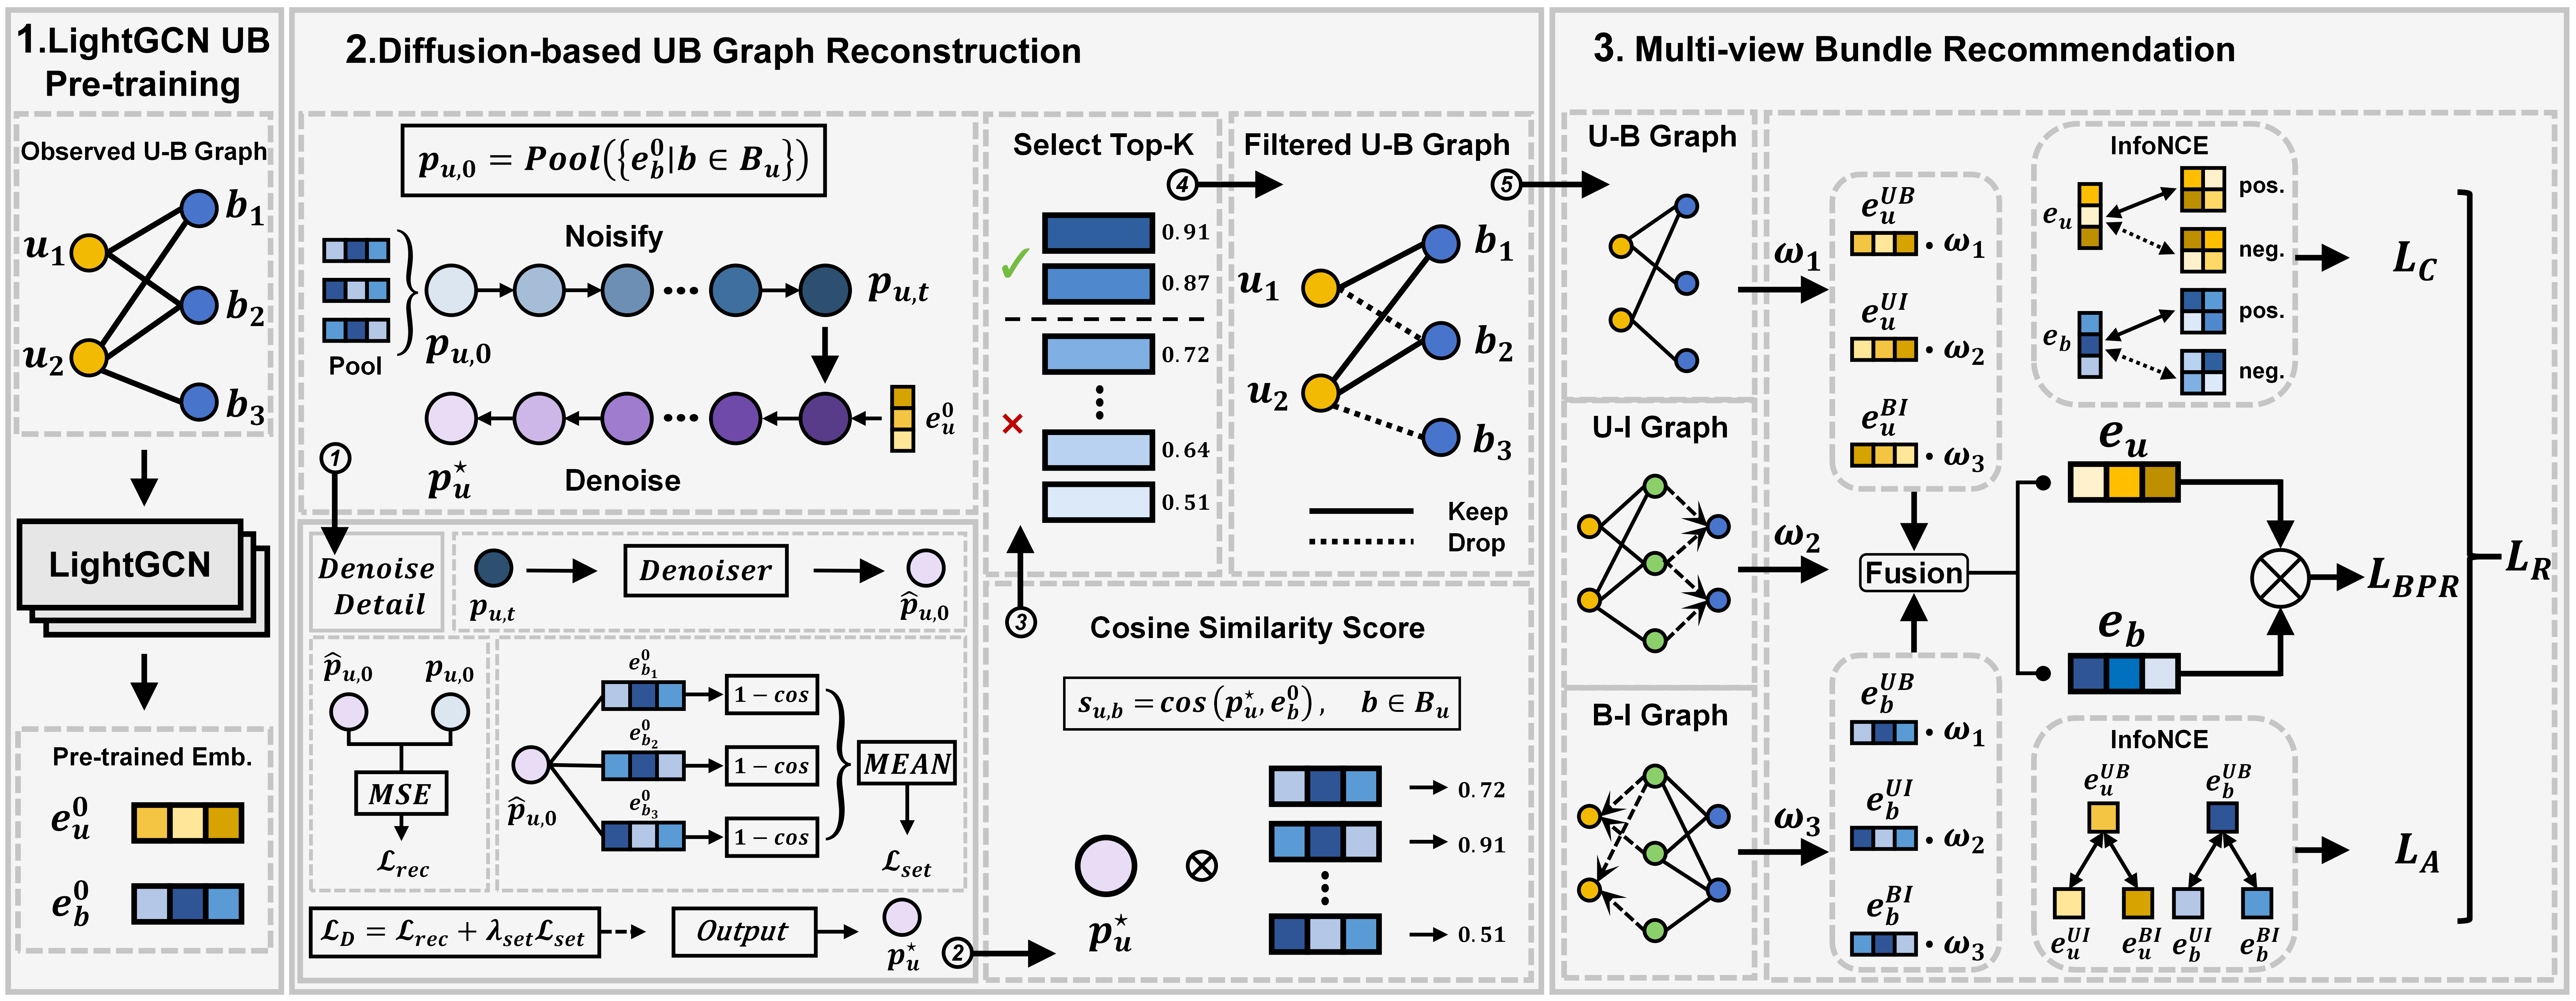
\includegraphics[width=0.98\textwidth]{Figures/digo_framework.png}
    \caption{Overall framework of ReCoBR, comprising U-B pretraining, diffusion-driven U-B graph reconstruction with user-conditioned denoising and bundle-set consistency, and multi-view recommendation with pre-fusion cross-view contrastive learning.}
    \label{fig:framework}
\end{figure*}


\section{Methodology}\label{sec:methodology}

\subsection{Task Definition and Framework Overview}

Let $\mathcal U$, $\mathcal B$, and $\mathcal I$ denote the sets of users, predefined bundles, and items, respectively. The available training data comprise three binary matrices: user-bundle interactions $\mathbf X\in\{0,1\}^{|\mathcal U|\times|\mathcal B|}$, user-item interactions $\mathbf Y\in\{0,1\}^{|\mathcal U|\times|\mathcal I|}$, and bundle-item affiliations $\mathbf Z\in\{0,1\}^{|\mathcal B|\times|\mathcal I|}$. In $\mathbf X$ and $\mathbf Y$, an entry equal to one denotes an observed interaction; in $\mathbf Z$, it denotes bundle membership. Given these relations, our task is to estimate a preference score $\hat y_{ub}$ for each unobserved user-bundle pair and rank candidate bundles for each user.

Figure~\ref{fig:framework} outlines ReCoBR. To address noise in U-B interactions, we first pretrain user and bundle representations, learn a user-conditioned denoiser over historical bundle representations, and use the refined preferences to reconstruct the U-B graph. The denoising objective incorporates a bundle-set consistency loss (SetLoss) to retain bundle-preference information during recovery. To address sparse U-B feedback, we then use the reconstructed U-B view as a common anchor for cross-view contrastive learning before representation fusion. The fused user and bundle representations produce the final recommendation scores.

We distinguish the observed matrix $\mathbf X$ from the reconstructed matrix $\widetilde{\mathbf X}$ throughout this section. The former defines users' training histories and ranking examples; the latter determines the U-B connections used for recommendation graph propagation.

\subsection{Diffusion-Driven U-B Graph Denoising and Reconstruction}\label{sec:graph-reconstruction}

The purpose of this module is to evaluate an observed interaction in the context of the user's historical bundle preferences. We construct this context in a pretrained representation space, refine it through conditional denoising, and translate the resulting preference vector into a selection of graph connections.

\subsubsection{Pretraining and Historical Preference Construction}

We pretrain LightGCN \cite{he2020lightgcn} on the observed U-B graph using Bayesian Personalized Ranking (BPR) \cite{rendle2009bpr}. Let $\mathbf h_u^{(0)},\mathbf h_b^{(0)}\in\mathbb R^d$ be its trainable initial embeddings, and let $\mathcal N_u=\{b\in\mathcal B:x_{ub}=1\}$ and $\mathcal N_b=\{u\in\mathcal U:x_{ub}=1\}$ denote the observed neighbors of user $u$ and bundle $b$. LightGCN propagation and layer aggregation are given by
\begin{equation}
\begin{aligned}
\mathbf h_u^{(\ell+1)}
&=\sum_{b\in\mathcal N_u}
\frac{\mathbf h_b^{(\ell)}}
{\sqrt{|\mathcal N_u||\mathcal N_b|}},\\
\mathbf h_b^{(\ell+1)}
&=\sum_{u\in\mathcal N_b}
\frac{\mathbf h_u^{(\ell)}}
{\sqrt{|\mathcal N_b||\mathcal N_u|}},\\
\mathbf e_u^0&=\sum_{\ell=0}^{L_p}\eta_\ell\mathbf h_u^{(\ell)},
\qquad
\mathbf e_b^0=\sum_{\ell=0}^{L_p}\eta_\ell\mathbf h_b^{(\ell)}.
\end{aligned}
\tag{1}
\end{equation}
Here, $L_p$ is the number of pretraining propagation layers, and the fixed aggregation coefficients satisfy $\eta_\ell\geq0$ and $\sum_{\ell=0}^{L_p}\eta_\ell=1$. The resulting embeddings $\mathbf e_u^0$ and $\mathbf e_b^0$ remain fixed during graph reconstruction. They are subsequently used to construct historical preferences, condition the denoiser, and score observed interactions.

For each active user $u$, we summarize the representations of the historically interacted bundles by mean pooling:
\begin{equation}
\mathbf p_{u,0}
=\frac{1}{|\mathcal N_u|}
\sum_{b\in\mathcal N_u}\mathbf e_b^0.
\tag{2}
\end{equation}
The vector $\mathbf p_{u,0}$ represents the user's observed bundle-preference context. Mean pooling accommodates histories of different lengths while keeping the denoising input $d$-dimensional. We construct this vector for users in $\mathcal U_+=\{u\in\mathcal U:|\mathcal N_u|>0\}$. The subscript $0$ denotes the state before artificial noise is added; it does not assume that the observed history is free of interaction noise.

\subsubsection{User-Conditioned Diffusion Denoising}

We train the denoiser to recover historical preference representations under different levels of perturbation. Following the Gaussian diffusion formulation \cite{ho2020ddpm,wang2023diffrec}, let $T$ be the number of diffusion steps and $\beta_t\in(0,1)$ the noise variance at step $t$. We use a linear variance schedule and define $\alpha_t=1-\beta_t$ and $\bar\alpha_t=\prod_{s=1}^{t}\alpha_s$. A perturbed preference vector can be sampled directly as
\begin{equation}
\mathbf p_{u,t}
=\sqrt{\bar\alpha_t}\,\mathbf p_{u,0}
+\sqrt{1-\bar\alpha_t}\,\boldsymbol\epsilon,
\qquad
\boldsymbol\epsilon\sim\mathcal N(\mathbf 0,\mathbf I_d).
\tag{3}
\end{equation}
Here, $\boldsymbol\epsilon\in\mathbb R^d$ is standard Gaussian noise, $\mathbf I_d$ is the $d$-dimensional identity matrix, and $\bar\alpha_t$ controls how much historical information remains at noise level $t$.

To make recovery personalized, we condition the denoiser on the pretrained user representation $\mathbf e_u^0$. We implement the denoiser $f_\theta$ as a multilayer perceptron (MLP), with parameters $\theta$, that predicts the unperturbed preference vector:
\begin{equation}
\begin{aligned}
\widehat{\mathbf p}_{u,0}
&=f_\theta(\mathbf p_{u,t},\mathbf e_u^0,t),\\
f_\theta(\mathbf p,\mathbf c,t)
&=\operatorname{MLP}_\theta
\bigl([\mathbf p;\mathbf c;\mathbf p\odot\mathbf c;
|\mathbf p-\mathbf c|;\boldsymbol\psi(t)]\bigr).
\end{aligned}
\tag{4}
\end{equation}
In Eq. (4), $[\cdot;\cdot]$ denotes concatenation, $\odot$ denotes element-wise multiplication, and $|\mathbf p-\mathbf c|$ is the element-wise absolute deviation. The vectors $\mathbf p$ and $\mathbf c$ preserve the current preference estimate and the user condition, while $\mathbf p\odot\mathbf c$ and $|\mathbf p-\mathbf c|$ expose their coordinate-wise agreement and discrepancy. The sinusoidal embedding $\boldsymbol\psi(t)\in\mathbb R^{d_t}$ specifies the perturbation level. Together with the timestep embedding, these features allow the MLP to adapt preference recovery to both the user and the perturbation level. Consequently, the MLP receives a $(4d+d_t)$-dimensional input and predicts a $d$-dimensional preference vector.

During training, we uniformly sample $u\in\mathcal U_+$ and $t\in\{1,\ldots,T\}$ and draw Gaussian noise as in Eq. (3). The reconstruction objective is
\begin{equation}
\mathcal L_{\mathrm{rec}}
=\mathbb E_{u,t,\boldsymbol\epsilon}
\left[
\frac{1}{d}
\left\|\widehat{\mathbf p}_{u,0}-\mathbf p_{u,0}\right\|_2^2
\right].
\tag{5}
\end{equation}
This objective learns a shared recovery function from perturbed historical preferences. The original representation supplies the reconstruction target, while the pretrained user embedding provides personalized context.

\subsubsection{Bundle-Set Consistency in Denoising}

Reconstructing the pooled vector provides a basic denoising objective, but subsequent interaction selection depends on the recovered vector's compatibility with individual historical bundles. We therefore introduce SetLoss to connect preference recovery with the bundle representations that will be used for graph reconstruction. Figure~\ref{fig:framework} illustrates how SetLoss complements the reconstruction objective in denoiser training.

Let $\operatorname{sim}(\mathbf a,\mathbf b)=\mathbf a^\top\mathbf b/(\|\mathbf a\|_2\|\mathbf b\|_2)$ denote cosine similarity, with a small numerical safeguard for zero norms. SetLoss encourages average directional agreement between the recovered preference and the user's historical bundle representations:
\begin{equation}
\mathcal L_{\mathrm{set}}
=\mathbb E_{u,t,\boldsymbol\epsilon}
\left[
\frac{1}{|\mathcal N_u|}
\sum_{b\in\mathcal N_u}
\left(1-\operatorname{sim}
\left(\widehat{\mathbf p}_{u,0},\mathbf e_b^0\right)\right)
\right].
\tag{6}
\end{equation}
Equation (5) reconstructs the pooled preference vector, whereas Eq. (6) aligns the recovered preference with its constituent historical bundles under the cosine-similarity geometry later used for interaction scoring. Averaging over the history prevents users with more interactions from dominating the objective.

We optimize the denoiser with
\begin{equation}
\mathcal L_{\mathrm D}
=\mathcal L_{\mathrm{rec}}
+\lambda_{\mathrm{set}}\mathcal L_{\mathrm{set}},
\tag{7}
\end{equation}
where $\lambda_{\mathrm{set}}\geq 0$ controls the contribution of SetLoss.

\subsubsection{Preference Refinement and Graph Reconstruction}

After learning the denoiser, we use it to refine the historical preference vector for interaction scoring. This stage employs a deterministic refinement procedure initialized with $\mathbf p_{u,0}$. Specifically,
\begin{equation}
\begin{aligned}
\mathbf r_{u,T}&=\mathbf p_{u,0},\\
\mathbf r_{u,t-1}
&=f_\theta(\mathbf r_{u,t},\mathbf e_u^0,t),
\qquad t=T,T-1,\ldots,1,\\
\mathbf p_u^\star&=\mathbf r_{u,0}.
\end{aligned}
\tag{8}
\end{equation}
The states $\mathbf r_{u,t}$ are refinement iterates, distinct from the forward-corrupted training states $\mathbf p_{u,t}$. Each iteration feeds the current estimate back into the denoiser with the next timestep condition. Thus, graph reconstruction applies the learned recovery network to an observed preference context, without sampling a Gaussian starting state.

We measure how closely each observed bundle matches the refined preference:
\begin{equation}
s_{ub}
=\operatorname{sim}(\mathbf p_u^\star,\mathbf e_b^0),
\qquad b\in\mathcal N_u.
\tag{9}
\end{equation}
For each user, we retain the highest-scoring $\kappa_u=\min(\kappa,|\mathcal N_u|)$ bundles, where the positive integer $\kappa$ controls the maximum retained degree:
\begin{equation}
\begin{aligned}
\widetilde{\mathcal N}_u
&=\underset{b\in\mathcal N_u}{\operatorname{TopK}}
\left(s_{ub},\kappa_u\right),\\
\widetilde x_{ub}
&=\mathbf 1\!\left[b\in\widetilde{\mathcal N}_u\right].
\end{aligned}
\tag{10}
\end{equation}
Here, $\operatorname{TopK}(s_{ub},\kappa_u)$ returns the set of $\kappa_u$ bundles in $\mathcal N_u$ with the largest scores, and $\mathbf 1[\cdot]$ is the indicator function. The dataset-specific value of $\kappa$ is reported in the experimental settings. Users with at most $\kappa$ observed bundles retain their full histories; users outside $\mathcal U_+$ have no retained U-B edges. Selection is restricted to observed interactions, so graph reconstruction neither creates new edges nor changes the ranking labels defined by $\mathbf X$. The resulting binary matrix $\widetilde{\mathbf X}$ is the reconstructed U-B graph used for downstream propagation.

\subsection{Pre-Fusion Cross-View Contrastive Learning}

With the U-B graph reconstructed, we next learn representations from this graph together with user-item behavior and bundle composition. The auxiliary relations provide complementary evidence when a user's bundle feedback is limited. We first construct user and bundle representations in each view, and then connect them through U-B-anchored contrastive learning before fusion.

\subsubsection{View-Specific Representations}

Following the three-view backbone of MultiCBR \cite{ma2024multicbr}, we construct the U-B, U-I, and B-I propagation graphs from $\widetilde{\mathbf X}$, $\mathbf Y$, and $\mathbf Z$, respectively. Each encoder applies $L$ layers of symmetrically normalized LightGCN-style propagation \cite{he2020lightgcn}. Fixed view-specific coefficients combine the initial embeddings with the $\ell_2$-normalized layer outputs. During training, the inherited backbone adds small representation perturbations to the propagation outputs and auxiliary item pooling; these perturbations are disabled during evaluation. The encoders share trainable initial embeddings for the same entity, which are separate from the fixed pretrained embeddings in Section~\ref{sec:graph-reconstruction}.

\textbf{U-B view.} Propagation on the reconstructed U-B graph directly produces user representations $\mathbf e_u^{\mathrm{UB}}$ and bundle representations $\mathbf e_b^{\mathrm{UB}}$, capturing collaborative information through the retained interactions.

\textbf{U-I view.} Propagation on the U-I graph produces user representations $\mathbf e_u^{\mathrm{UI}}$ and item representations $\mathbf e_i^{\mathrm{UI}}$. To obtain a bundle representation $\mathbf e_b^{\mathrm{UI}}$ in this view, we average the representations of its constituent items according to $\mathbf Z$.

\textbf{B-I view.} Propagation on the B-I graph produces bundle representations $\mathbf e_b^{\mathrm{BI}}$ and item representations $\mathbf e_i^{\mathrm{BI}}$. To obtain a user representation $\mathbf e_u^{\mathrm{BI}}$ in this view, we average the representations of the items that the user has interacted with according to $\mathbf Y$.

The two item-pooling operations are
\begin{equation}
\mathbf e_b^{\mathrm{UI}}
=\frac{1}{|\mathcal I_b|}
\sum_{i\in\mathcal I_b}\mathbf e_i^{\mathrm{UI}},
\qquad
\mathbf e_u^{\mathrm{BI}}
=\frac{1}{|\mathcal I_u|}
\sum_{i\in\mathcal I_u}\mathbf e_i^{\mathrm{BI}},
\tag{11}
\end{equation}
where $\mathcal I_b=\{i:z_{bi}=1\}$ contains the items in bundle $b$, and $\mathcal I_u=\{i:y_{ui}=1\}$ contains the items interacted with by user $u$. An empty neighborhood contributes a zero vector.

This step yields three representations for each user, $\{\mathbf e_u^{\mathrm{UB}},\mathbf e_u^{\mathrm{UI}},\mathbf e_u^{\mathrm{BI}}\}$, and each bundle, $\{\mathbf e_b^{\mathrm{UB}},\mathbf e_b^{\mathrm{UI}},\mathbf e_b^{\mathrm{BI}}\}$, all in $\mathbb R^d$. These unfused representations are used to construct the cross-view objective below and are later fused for prediction.

\subsubsection{Cross-View Objectives Anchored in U-B}

Using these view-specific representations, we pair each user's U-B representation with its U-I and B-I counterparts, and do the same for each bundle. The reconstructed U-B view thus serves as the common reference. Each same-entity pair is a positive pair, while other entities of the same type provide in-batch negatives. For every recommendation minibatch, we remove duplicate user IDs and duplicate positive-bundle IDs to form the entity sets $\mathcal S_U$ and $\mathcal S_B$, ensuring that an entity is not repeated as its own in-batch negative.

For two views $v$ and $w$ and an entity set $\mathcal S$, we define the directional InfoNCE objective \cite{oord2018cpc} as
\begin{equation}
\ell_\tau^{v,w}(\mathcal S)
=-\frac{1}{|\mathcal S|}\sum_{q\in\mathcal S}
\log
\frac{\exp\!\left(\operatorname{sim}(\mathbf e_q^v,\mathbf e_q^w)/\tau\right)}
{\sum_{q'\in\mathcal S}
\exp\!\left(\operatorname{sim}(\mathbf e_q^v,\mathbf e_{q'}^w)/\tau\right)}.
\tag{12}
\end{equation}
The temperature $\tau>0$ controls sensitivity to similarity differences. For each anchor $\mathbf e_q^v$, its counterpart $\mathbf e_q^w$ is the positive candidate, and the representations of all entities in $\mathcal S$, including the positive, form the denominator. The pre-fusion objective is
\begin{equation}
\begin{aligned}
\mathcal L_{\mathrm A}
={}&\ell_\tau^{\mathrm{UB},\mathrm{UI}}(\mathcal S_U)
+\ell_\tau^{\mathrm{UB},\mathrm{BI}}(\mathcal S_U)\\
&+\ell_\tau^{\mathrm{UB},\mathrm{UI}}(\mathcal S_B)
+\ell_\tau^{\mathrm{UB},\mathrm{BI}}(\mathcal S_B).
\end{aligned}
\tag{13}
\end{equation}
Equation (13) encourages agreement for the same user or bundle across U-B--U-I and U-B--B-I pairs while preserving discrimination between entities. A user-side or bundle-side term is omitted when the corresponding entity set contains fewer than two members and therefore provides no in-batch negatives. The U-B view is the common anchor in constructing the objective, and gradients update both representations in each pair. These constraints inject behavioral and compositional evidence into bundle-level preference learning when U-B histories are sparse.

\subsection{Prediction and Model Optimization}

\textbf{View fusion and prediction.} Following MultiCBR \cite{ma2024multicbr}, we adopt its fixed view coefficients to combine the three view-specific representations into a single user representation and a single bundle representation. Their inner product gives the preference score:
\begin{equation}
\begin{aligned}
\mathbf e_u
&=\omega_1\mathbf e_u^{\mathrm{UB}}
+\omega_2\mathbf e_u^{\mathrm{UI}}
+\omega_3\mathbf e_u^{\mathrm{BI}},\\
\mathbf e_b
&=\omega_1\mathbf e_b^{\mathrm{UB}}
+\omega_2\mathbf e_b^{\mathrm{UI}}
+\omega_3\mathbf e_b^{\mathrm{BI}},\\
\hat y_{ub}&=\mathbf e_u^\top\mathbf e_b.
\end{aligned}
\tag{14}
\end{equation}
Here, $\omega_1$, $\omega_2$, and $\omega_3$ are fixed coefficients for the U-B, U-I, and B-I views, respectively. The same coefficients are used for users and bundles; they are nonnegative and satisfy $\omega_1+\omega_2+\omega_3=1$. Their dataset-specific values are reported in the experimental settings.

\textbf{Recommendation objectives.} Let $\mathcal Q$ be a minibatch of $m$ ranking triplets, indexed as $(u_j,b_j^+,b_j^-)$ for $j=1,\ldots,m$. Here, $x_{u_jb_j^+}=1$ and $b_j^-\in\mathcal B\setminus\mathcal N_{u_j}$. Following MultiCBR \cite{ma2024multicbr}, the fused-space self-contrastive regularizer is
\begin{equation}
\begin{aligned}
\mathcal L_{\mathrm C}
=-\frac{1}{2m}\sum_{j=1}^{m}\Bigg[
&\log\frac{\exp\!\left(\operatorname{sim}(\mathbf e_{u_j},\mathbf e_{u_j})/\tau\right)}
{\sum_{k=1}^{m}\exp\!\left(\operatorname{sim}(\mathbf e_{u_j},\mathbf e_{u_k})/\tau\right)}\\
+&\log\frac{\exp\!\left(\operatorname{sim}(\mathbf e_{b_j^+},\mathbf e_{b_j^+})/\tau\right)}
{\sum_{k=1}^{m}\exp\!\left(\operatorname{sim}(\mathbf e_{b_j^+},\mathbf e_{b_k^+})/\tau\right)}
\Bigg].
\end{aligned}
\tag{15}
\end{equation}
For each occurrence in the minibatch, the numerator pairs its fused representation with itself, while all minibatch occurrences of the same entity type appear in the denominator. This inherited objective regularizes separation in the fused representation space, whereas $\mathcal L_{\mathrm A}$ explicitly connects different relation views before fusion. We optimize BPR \cite{rendle2009bpr} together with the two regularization objectives:
\begin{equation}
\begin{aligned}
\mathcal L_{\mathrm{BPR}}
&=-\frac{1}{m}
\sum_{j=1}^{m}
\log\sigma\!\left(\hat y_{u_jb_j^+}-\hat y_{u_jb_j^-}\right),\\
\mathcal L_{\mathrm R}
&=\mathcal L_{\mathrm{BPR}}
+\lambda_a\mathcal L_{\mathrm A}
+\lambda_c\mathcal L_{\mathrm C}
+\lambda_r\|\Theta\|_2^2.
\end{aligned}
\tag{16}
\end{equation}
Here, $\sigma$ is the sigmoid function, $\Theta$ comprises the trainable initial user, bundle, and item embeddings of the recommendation backbone, and $\lambda_a,\lambda_c,\lambda_r\geq0$ balance the loss terms. Ranking examples continue to come from $\mathbf X$, even when their edges are not selected for $\widetilde{\mathbf X}$. Graph reconstruction therefore filters propagation connections while preserving the observed feedback used for ranking.

\textbf{Training.} After offline U-B pretraining, each training epoch contains three stages. First, we update the denoiser $f_\theta$ for one pass over $\mathcal U_+$ using $\mathcal L_{\mathrm D}$. Second, the updated denoiser refines every active user's historical preference, scores the observed U-B interactions, and refreshes $\widetilde{\mathbf X}$ through the Top-K selection in Eq. (10). Third, we hold $\widetilde{\mathbf X}$ fixed and update the recommendation parameters $\Theta$ on ranking minibatches using $\mathcal L_{\mathrm R}$. The denoiser and recommendation backbone use separate optimizers. Because Top-K edge selection is discrete, gradients from $\mathcal L_{\mathrm R}$ do not propagate through $\widetilde{\mathbf X}$ to $f_\theta$.

\textbf{Inference.} Using the reconstructed graph associated with the selected model, we compute and cache the three view-specific representations and their fused user and bundle embeddings. For each user, we rank candidate bundles by Eq. (14) after excluding bundles observed in the training data. Graph reconstruction is performed before scoring; the denoiser is not run separately for each candidate bundle.

\subsection{Computational Complexity}

Let $n_+=|\mathcal U_+|$ and $h_{\max}=\max_{u\in\mathcal U_+}|\mathcal N_u|$. Let $M=|\mathcal E_{\mathrm{UB}}|$ be the number of observed U-B edges, and let $E=|\widetilde{\mathcal E}_{\mathrm{UB}}|+|\mathcal E_{\mathrm{UI}}|+|\mathcal E_{\mathrm{BI}}|$ be the total number of edges used for graph propagation. We use $Q$ and $m$ to denote the number and size of recommendation minibatches, respectively. With a fixed-depth denoiser whose hidden widths scale with $d$, one evaluation costs $C_f=O(d^2)$. The time complexity of one training epoch is

\begin{equation}
O\!\left(
\begin{aligned}
&(T+1)n_+C_f\\
&+n_+h_{\max}\!\left[d+\log(1+\kappa)\right]\\
&+Q\bigl(LEd+m^2d\bigr)
\end{aligned}
\right).
\tag{17}
\end{equation}
The three terms correspond to denoiser training and refinement, history processing and bounded-heap Top-K graph reconstruction, and recommendation learning, respectively. Offline LightGCN pretraining requires $O(L_pMd)$ per propagation pass. Since $|\widetilde{\mathcal E}_{\mathrm{UB}}|\leq M$, reconstruction does not densify the U-B graph.

For space complexity, let $V=|\mathcal U|+|\mathcal B|+|\mathcal I|$, let $b_d$ be the maximum denoising or reconstruction batch size, and let $P_\theta$ be the denoiser parameter count. The peak training space is
\begin{equation}
O\!\left(
\begin{aligned}
&(L+1)Vd+P_\theta+(|\mathcal U|+|\mathcal B|)d\\
&+E+M+m^2+b_dh_{\max}d
\end{aligned}
\right).
\tag{18}
\end{equation}
At inference, constructing the cached graph representations costs $O(LEd)$. Scoring one user-bundle pair costs $O(d)$, and ranking all candidate bundles for one user costs $O(|\mathcal B|d)$.


\section{Experiments}

We evaluate ReCoBR on three bundle recommendation benchmarks.
The experiments examine its overall ranking performance, the
contributions of graph reconstruction and pre-fusion cross-view
learning, and their behavior under different interaction
selection strategies and levels of user feedback. We also
analyze sensitivity to the key hyperparameters.

% =========================================================
% Table 1: Dataset statistics, single-column table
% =========================================================
% Prefer placement here, within Experiments, before allowing a top float.
\begin{table}[!ht]
    \centering
    {\small
    \setlength{\tabcolsep}{2pt}
    \begin{tabular}{@{}lrrrrrr@{}}
        \toprule
        Dataset
        & \#Users
        & \#Items
        & \#Bundles
        & \#U--I
        & \#U--B
        & \shortstack{\#Avg.\\I/B} \\
        \midrule
        Youshu
        & 8,039
        & 32,770
        & 4,771
        & 138,515
        & 51,377
        & 37.03 \\
        NetEase
        & 18,528
        & 123,628
        & 22,864
        & 1,128,065
        & 302,303
        & 77.80 \\
        iFashion
        & 53,897
        & 42,563
        & 27,694
        & 2,290,645
        & 1,679,708
        & 3.86 \\
        \bottomrule
    \end{tabular}
    }

    \caption{Dataset statistics. U--I and U--B count user--item
    and user--bundle interactions; Avg. I/B is the average
    number of items per bundle.}
    \label{tab:datasets}
\end{table}


% =========================================================
% Table 2: Overall results, double-column table
% =========================================================
\begin{table*}[t]
    \centering
    {\small
    \setlength{\tabcolsep}{1mm}
    \begin{tabular}{@{}lrrrrrrrrrrrr@{}}
        \toprule
        \multirow{2}{*}{Method}
        & \multicolumn{4}{c}{Youshu}
        & \multicolumn{4}{c}{iFashion}
        & \multicolumn{4}{c}{NetEase} \\
        \cmidrule(lr){2-5}
        \cmidrule(lr){6-9}
        \cmidrule(lr){10-13}
        & R@20 & N@20 & R@40 & N@40
        & R@20 & N@20 & R@40 & N@40
        & R@20 & N@20 & R@40 & N@40 \\
        \midrule

        BGCN
        & 0.2436 & 0.1329 & 0.3379 & 0.1589
        & 0.0802 & 0.0582 & 0.1239 & 0.0736
        & 0.0626 & 0.0328 & 0.0988 & 0.0424 \\

        MIDGN
        & 0.2682 & 0.1527 & 0.3712 & 0.1808
        & 0.0856 & 0.0473 & 0.1299 & 0.0593
        & 0.0678 & 0.0343 & 0.1085 & 0.0451 \\

        CrossCBR
        & 0.2823 & 0.1670 & 0.3787 & 0.1939
        & 0.1132 & 0.0872 & 0.1623 & 0.1045
        & 0.0844 & 0.0458 & 0.1255 & 0.0567 \\

        BundleGT
        & \underline{0.2905} & \underline{0.1737} & 0.3909 & \underline{0.2011}
        & 0.1263 & 0.0969 & 0.1819 & 0.1164
        & 0.0903 & 0.0478 & \underline{0.1389} & 0.0606 \\

        MultiCBR
        & 0.2842 & 0.1693 & 0.3946 & 0.1994
        & \underline{0.1500} & \underline{0.1203} & \underline{0.2033} & \underline{0.1390}
        & 0.0907 & 0.0494 & 0.1355 & 0.0612 \\

        EBRec
        & 0.2858 & 0.1701 & 0.3871 & 0.1979
        & 0.1329 & 0.1047 & 0.1873 & 0.1238
        & 0.0899 & 0.0487 & 0.1359 & 0.0604 \\

        EpicCBR
        & 0.2852 & 0.1691 & \underline{0.3949} & 0.1985
        & -- & -- & -- & --
        & \underline{0.0913} & \underline{0.0502} & 0.1345 & \underline{0.0615} \\

        \textbf{ReCoBR}
        & \textbf{0.2920} & \textbf{0.1759} & \textbf{0.3997} & \textbf{0.2023}
        & \textbf{0.1568} & \textbf{0.1315} & \textbf{0.2067} & \textbf{0.1491}
        & \textbf{0.0955} & \textbf{0.0511} & \textbf{0.1390} & \textbf{0.0627} \\

        \midrule
        \textbf{Improv.}
        & \textbf{0.52\%} & \textbf{1.27\%} & \textbf{1.22\%} & \textbf{0.60\%}
        & \textbf{4.53\%} & \textbf{9.31\%} & \textbf{1.67\%} & \textbf{7.27\%}
        & \textbf{4.60\%} & \textbf{1.79\%} & \textbf{0.07\%} & \textbf{1.95\%} \\
        \bottomrule
    \end{tabular}
    }

    \caption{Overall performance at Top-20 and Top-40 on three
    datasets. R and N denote Recall and NDCG. Bold and underlined
    entries mark the best and second-best reported results,
    respectively. Improv. is ReCoBR's relative improvement over
    the strongest reported baseline for each metric; dashes
    indicate results not yet reported.}
    \label{tab:overall}
\end{table*}


% Table 3: Ablation study, single-column table
% =========================================================
\begin{table}[t]
    \centering
    {\small
    \setlength{\tabcolsep}{2pt}
    \begin{tabular}{@{}lrrrrrr@{}}
        \toprule
        \multirow{2}{*}{Variant}
        & \multicolumn{2}{c}{Youshu}
        & \multicolumn{2}{c}{NetEase}
        & \multicolumn{2}{c}{iFashion} \\
        \cmidrule(lr){2-3}
        \cmidrule(lr){4-5}
        \cmidrule(lr){6-7}
        & R@20 & N@20
        & R@20 & N@20
        & R@20 & N@20 \\
        \midrule

        \textbf{ReCoBR}
        & \textbf{0.2920}
        & \textbf{0.1759}
        & \textbf{0.0955}
        & \textbf{0.0511}
        & \textbf{0.1568}
        & \textbf{0.1315} \\

        \shortstack[l]{w/o Graph\\Recon.}
        & 0.2919 & 0.1734
        & 0.0948 & 0.0509
        & 0.1500 & 0.1245 \\

        w/o SetLoss
        & 0.2913 & 0.1749
        & 0.0951 & 0.0506
        & 0.1559 & 0.1301 \\

        w/o All CL
        & 0.2326 & 0.1307
        & 0.0512 & 0.0260
        & 0.0400 & 0.0281 \\

        \shortstack[l]{w/o Pre-fusion\\CL}
        & 0.2901 & 0.1692
        & 0.0906 & 0.0487
        & 0.1558 & 0.1304 \\

        \shortstack[l]{w/o Post-fusion\\CL}
        & 0.2595 & 0.1502
        & 0.0682 & 0.0350
        & 0.0461 & 0.0350 \\
        \bottomrule
    \end{tabular}
    }

    \caption{Component ablations on three datasets, evaluated by
    Recall@20 (R@20) and NDCG@20 (N@20). Bold entries identify
    the complete ReCoBR model.}
    \label{tab:ablation}
\end{table}


\subsection{Experimental Settings}

\paragraph{Datasets and Evaluation.}
We use Youshu, NetEase, and iFashion for book-list, music-playlist,
and outfit recommendation, respectively. Each dataset contains
U-B interactions, U-I interactions, and B-I affiliations.
Table~\ref{tab:datasets} summarizes their statistics. We adopt
the preprocessed datasets and splits used by CrossCBR and
MultiCBR~\cite{ma2022crosscbr,ma2024multicbr}, with 70\%, 10\%, and
20\% of U-B interactions assigned to training, validation, and
testing. Pretraining, historical preference construction, and
U-B graph reconstruction use only the training interactions.

We report Recall@$K$ and NDCG@$K$ for $K\in\{20,40\}$ under
full-ranking evaluation. For each user, we rank all candidate
bundles after excluding those observed in training. The
checkpoint with the best Top-20 validation performance is
selected for test evaluation.

\paragraph{Baselines.}
We compare ReCoBR with seven bundle recommendation methods.
BGCN~\cite{chang2020bgcn} models bundle-level and item-level collaborative
information through graph propagation, while MIDGN~\cite{zhao2022midgn}
disentangles user intents across global and local views.
CrossCBR~\cite{ma2022crosscbr} connects bundle-view and item-view
representations through contrastive learning, and
BundleGT~\cite{wei2023bundlegt} uses a hierarchical graph Transformer
to model bundling strategies. MultiCBR~\cite{ma2024multicbr}
encodes all three relations and applies contrastive learning
after view fusion. EBRec~\cite{du2025ebrec} enhances item-level bundle
representations through bundle--user--item correlations.
EpicCBR~\cite{li2026epiccbr} combines item-relation enhancement with
contrastive learning across warm-start and cold-start scenarios.

The results of BGCN, MIDGN, CrossCBR, and MultiCBR are taken
from MultiCBR~\cite{ma2024multicbr}. For BundleGT and EBRec,
we use the results reported in their respective
papers~\cite{wei2023bundlegt,du2025ebrec}. We reproduce EpicCBR
using its released implementation under the same data splits
and evaluation protocol as ReCoBR.

\paragraph{Implementation Details.}
We implement ReCoBR in PyTorch and train it on a single NVIDIA
GeForce RTX 3090 GPU. The recommendation embeddings use Xavier
initialization, dimension 64, and two graph propagation layers.
We use Adam with a learning rate of $10^{-3}$, a recommendation
batch size of 2048, and one negative bundle per positive
interaction. Ranking examples are drawn from the original
training interactions; the reconstructed U-B graph determines
the propagation connections.

The denoiser is a two-layer MLP with hidden dimension 128,
timestep embedding dimension 16, and dropout rate 0.1. Its
separate optimizer uses a learning rate of $10^{-3}$, weight
decay $10^{-5}$, and batch size 1024. We use a linear noise
schedule from $\beta_1=10^{-4}$ to $\beta_T=0.02$. In the order
Youshu, NetEase, and iFashion, the diffusion steps $T$ are
$(9,12,12)$, the retention limits $\kappa$ are $(7,13,3)$, and
the SetLoss weights $\lambda_{\mathrm{set}}$ are
$(0.04,0.05,0.05)$.

The fixed fusion coefficients $(\omega_1,\omega_2,\omega_3)$,
corresponding to U-B, U-I, and B-I, are $(0.35,0.15,0.50)$
for Youshu, $(0.50,0.20,0.30)$ for NetEase, and
$(0.00,0.50,0.50)$ for iFashion. A zero U-B fusion coefficient
removes its direct contribution to the final weighted sum;
the U-B view still participates in pre-fusion contrastive
learning. In the same dataset order, the pre-fusion loss
weights $\lambda_a$ are $(0.004,0.005,0.07)$, and the
post-fusion loss weights $\lambda_c$ are $(0.04,0.05,0.10)$.
The shared contrastive temperature is $\tau=0.20$ on all three
datasets. The embedding regularization coefficient
$\lambda_r$ is $10^{-5}$. Hyperparameters are selected using
validation performance. We report the average ReCoBR performance
over three independent runs.


\subsection{Overall Performance}

Table~\ref{tab:overall} reports Top-20 and Top-40 results for
ReCoBR and seven baselines, with unavailable results marked by
dashes. ReCoBR obtains the highest reported Recall and NDCG
at both cutoffs on all three datasets. The strongest baseline
varies by dataset and metric. At Top-20, it is BundleGT on
Youshu, MultiCBR on iFashion, and EpicCBR on NetEase. At
Top-40, EpicCBR leads in Recall on Youshu and NDCG on NetEase,
BundleGT leads in NDCG on Youshu and Recall on NetEase,
and MultiCBR leads in both metrics on iFashion.

Compared with the strongest reported baseline for each metric,
ReCoBR improves R@20 and N@20 by 0.52\% and 1.27\% on Youshu,
4.53\% and 9.31\% on iFashion, and 4.60\% and 1.79\% on
NetEase, respectively. At Top-40, the corresponding improvements
are 1.22\% and 0.60\% on Youshu, 1.67\% and 7.27\% on
iFashion, and 0.07\% and 1.95\% on NetEase. The gain in
Recall@40 on NetEase is small, whereas the NDCG gain is larger.
EpicCBR's iFashion results remain to be reported.

The comparison with MultiCBR is particularly informative
because it already uses the three relation views, representation
fusion, and post-fusion contrastive learning. ReCoBR improves
over this baseline at both cutoffs on all three datasets. This
motivates examining the additional graph reconstruction and
pre-fusion objectives separately, as we do next, to understand
their contributions beyond the multi-view backbone.


\subsection{Ablation Study}

Table~\ref{tab:ablation} compares ReCoBR with five variants.
\textbf{w/o Graph Recon.} replaces the reconstructed U-B graph
with the original observed graph while retaining the
recommendation objectives. \textbf{w/o Pre-fusion CL} removes
the U-B-anchored cross-view objective but retains graph
reconstruction. \textbf{w/o Post-fusion CL} removes the
contrastive regularizer in the fused representation space,
and \textbf{w/o All CL} removes both contrastive objectives.

\paragraph{U-B Graph Reconstruction.}
Removing graph reconstruction reduces R@20 and N@20 on iFashion
from 0.1568 and 0.1315 to 0.1500 and 0.1245, respectively.
Both metrics also decrease on NetEase. On Youshu, R@20 is
essentially unchanged (0.2920 versus 0.2919), whereas N@20
drops from 0.1759 to 0.1734. Thus, the benefit of reconstruction
varies across datasets and metrics, with the clearest gains on
iFashion. These results support refining the U-B connections
used for propagation through the complete pretraining,
conditional denoising, and interaction-selection pipeline.

\paragraph{Bundle-Set Consistency.}
We additionally examine \textbf{w/o SetLoss}, which removes
the bundle-set consistency term from denoiser training while
retaining the reconstruction objective and both ReCoBR modules.
Removing this term yields a modest performance decrease
across all three datasets. This supports its role as an
auxiliary task-specific constraint: maintaining agreement
with historical bundle representations helps the recovered
preference serve subsequent interaction scoring.

\paragraph{Pre-Fusion Cross-View Learning.}
Removing the pre-fusion objective lowers both metrics on all
three datasets. On NetEase, R@20 and N@20 decrease from
0.0955 and 0.0511 to 0.0906 and 0.0487, respectively; on
Youshu, N@20 falls from 0.1759 to 0.1692. These comparisons
show that explicit U-B--U-I and U-B--B-I associations provide
value beyond representation fusion and its existing
regularizer. Using the reconstructed U-B view as a common
reference allows auxiliary behavioral and compositional
information to contribute to bundle-preference learning
before the views are combined.

\paragraph{Backbone Contrastive Regularization.}
Removing post-fusion contrastive learning causes larger
decreases, and removing both contrastive objectives further
reduces performance on every dataset. The fused-space
regularizer therefore remains important to the inherited
recommendation backbone. Meanwhile, the full model's gains
over \textbf{w/o Pre-fusion CL} show that this regularizer does
not make the proposed cross-view objective redundant. The
two objectives constrain different representations:
relation-specific pairs before fusion and the combined
representations used for prediction.


\subsection{In-depth Analysis}

\begin{figure}[t]
    \centering
    \begin{tabular}{@{}cc@{}}
        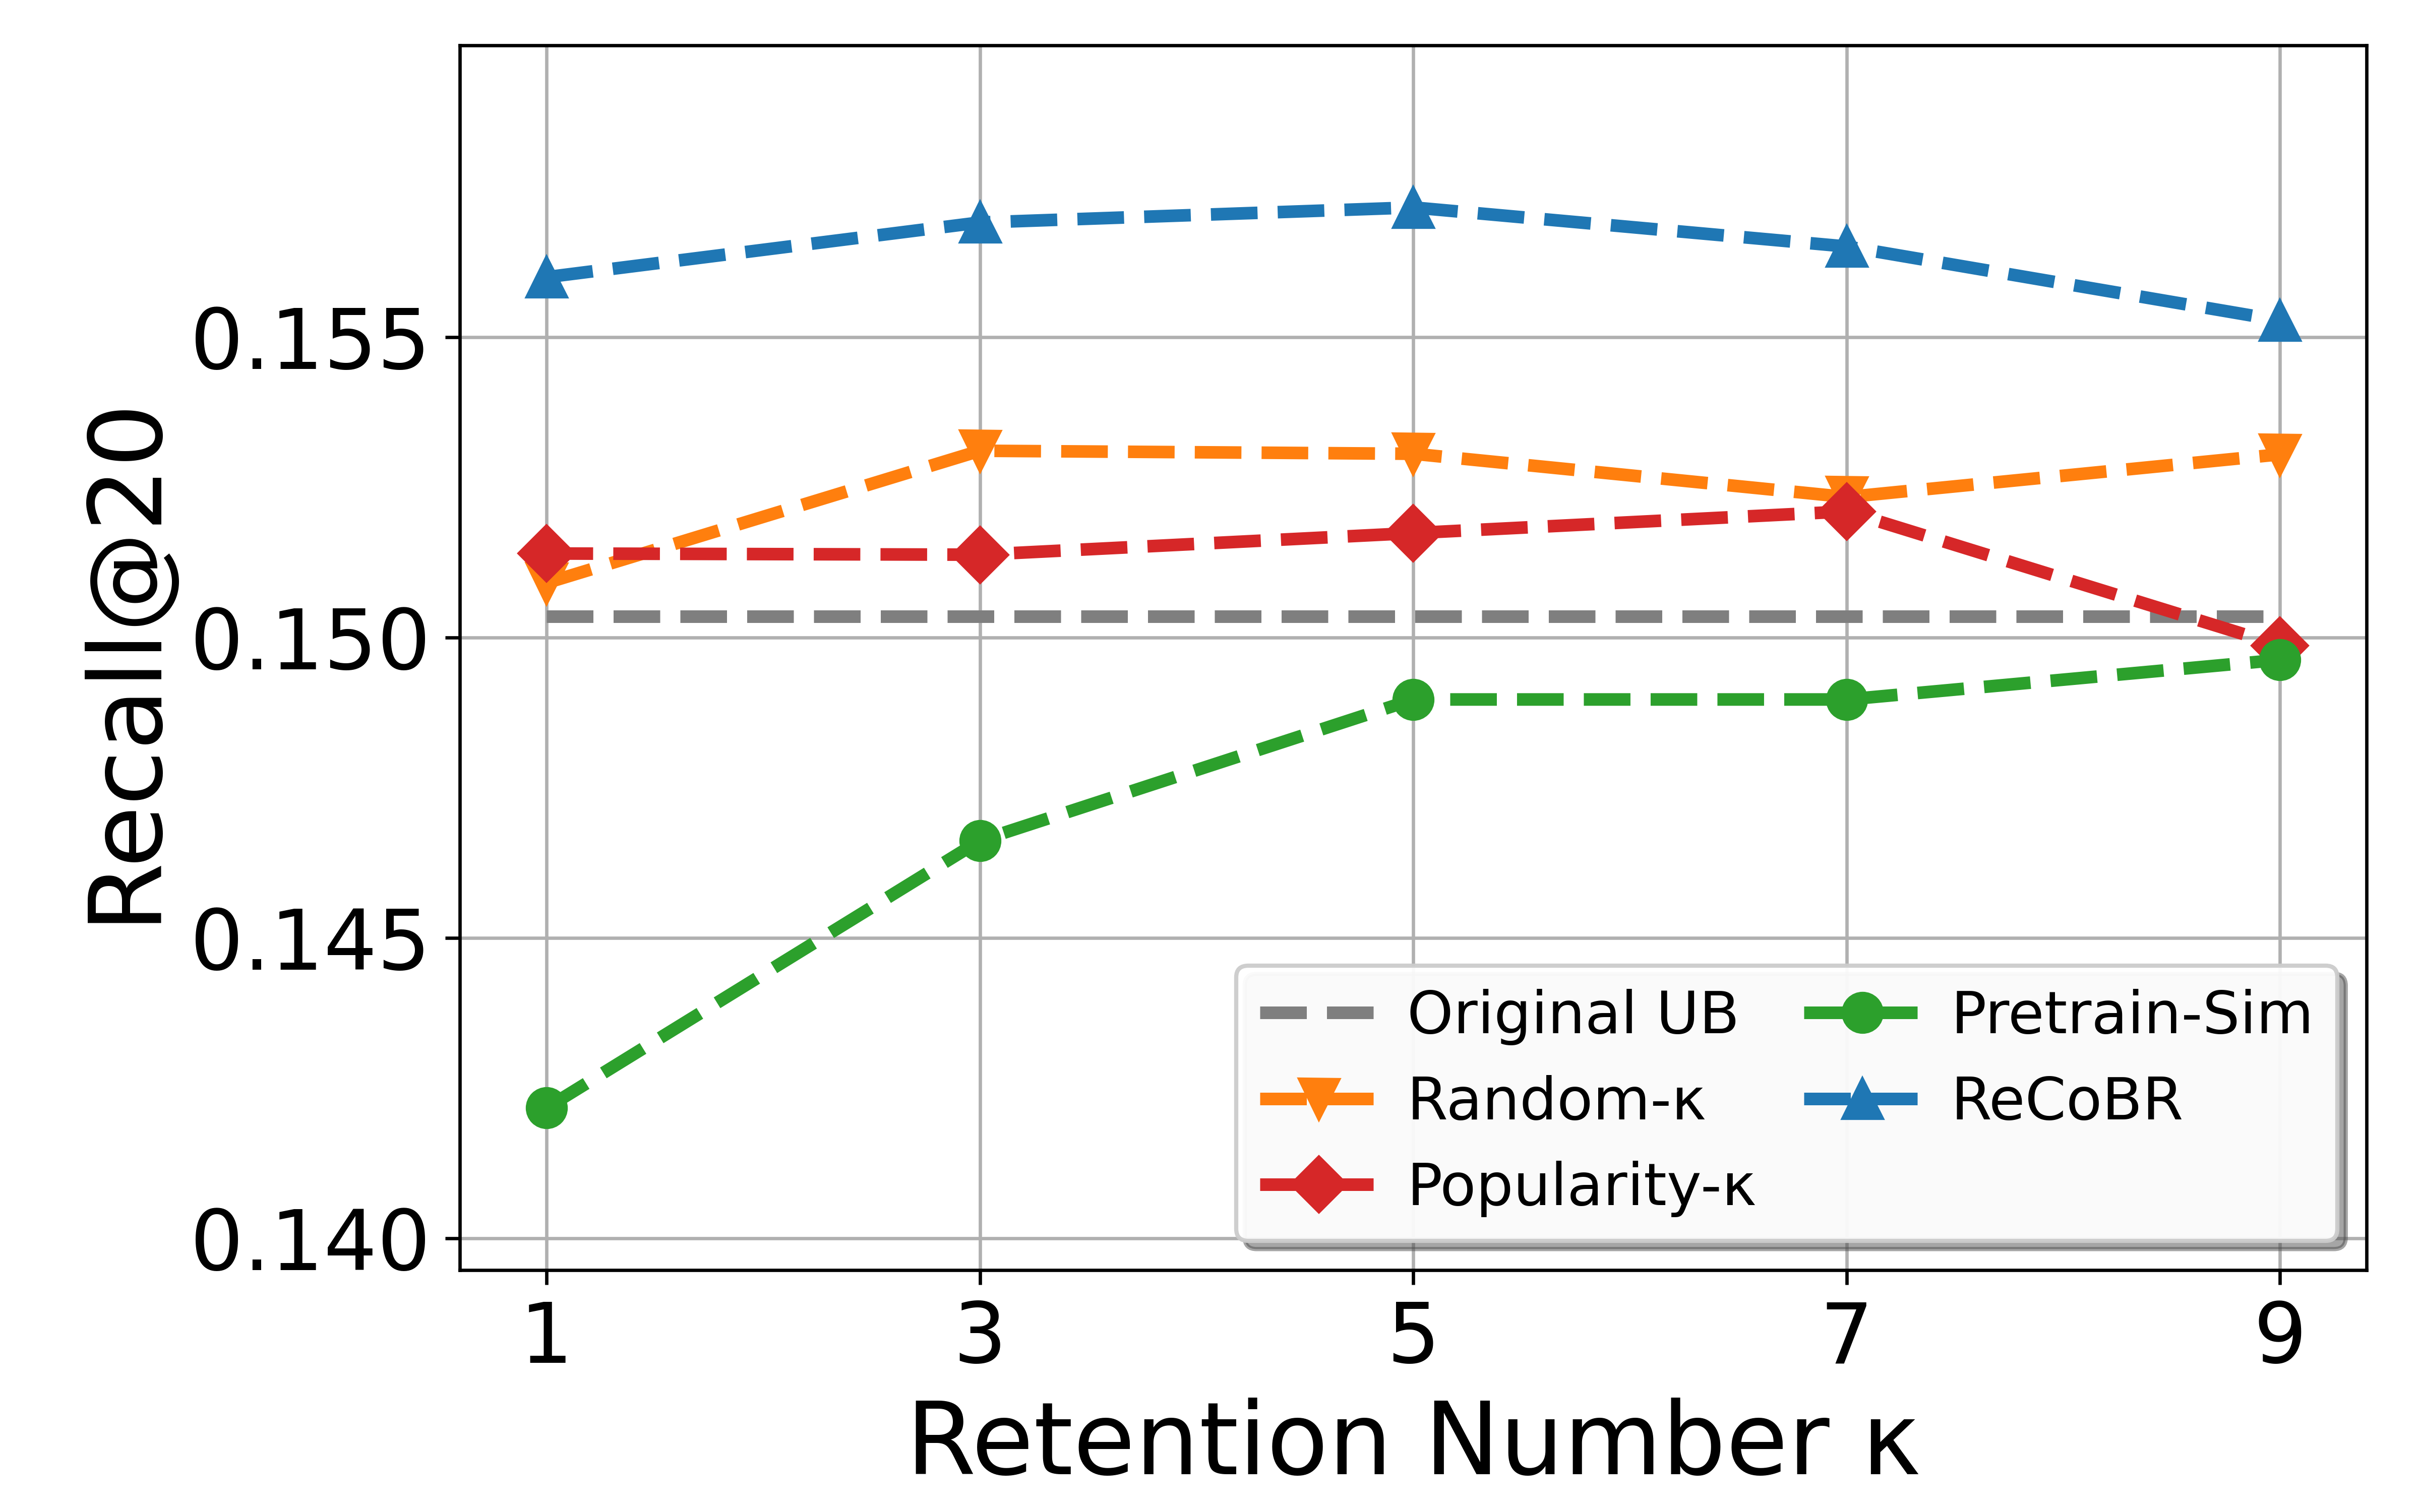
\includegraphics[width=0.46\columnwidth]
        {Figures/m1recall20.png} &
        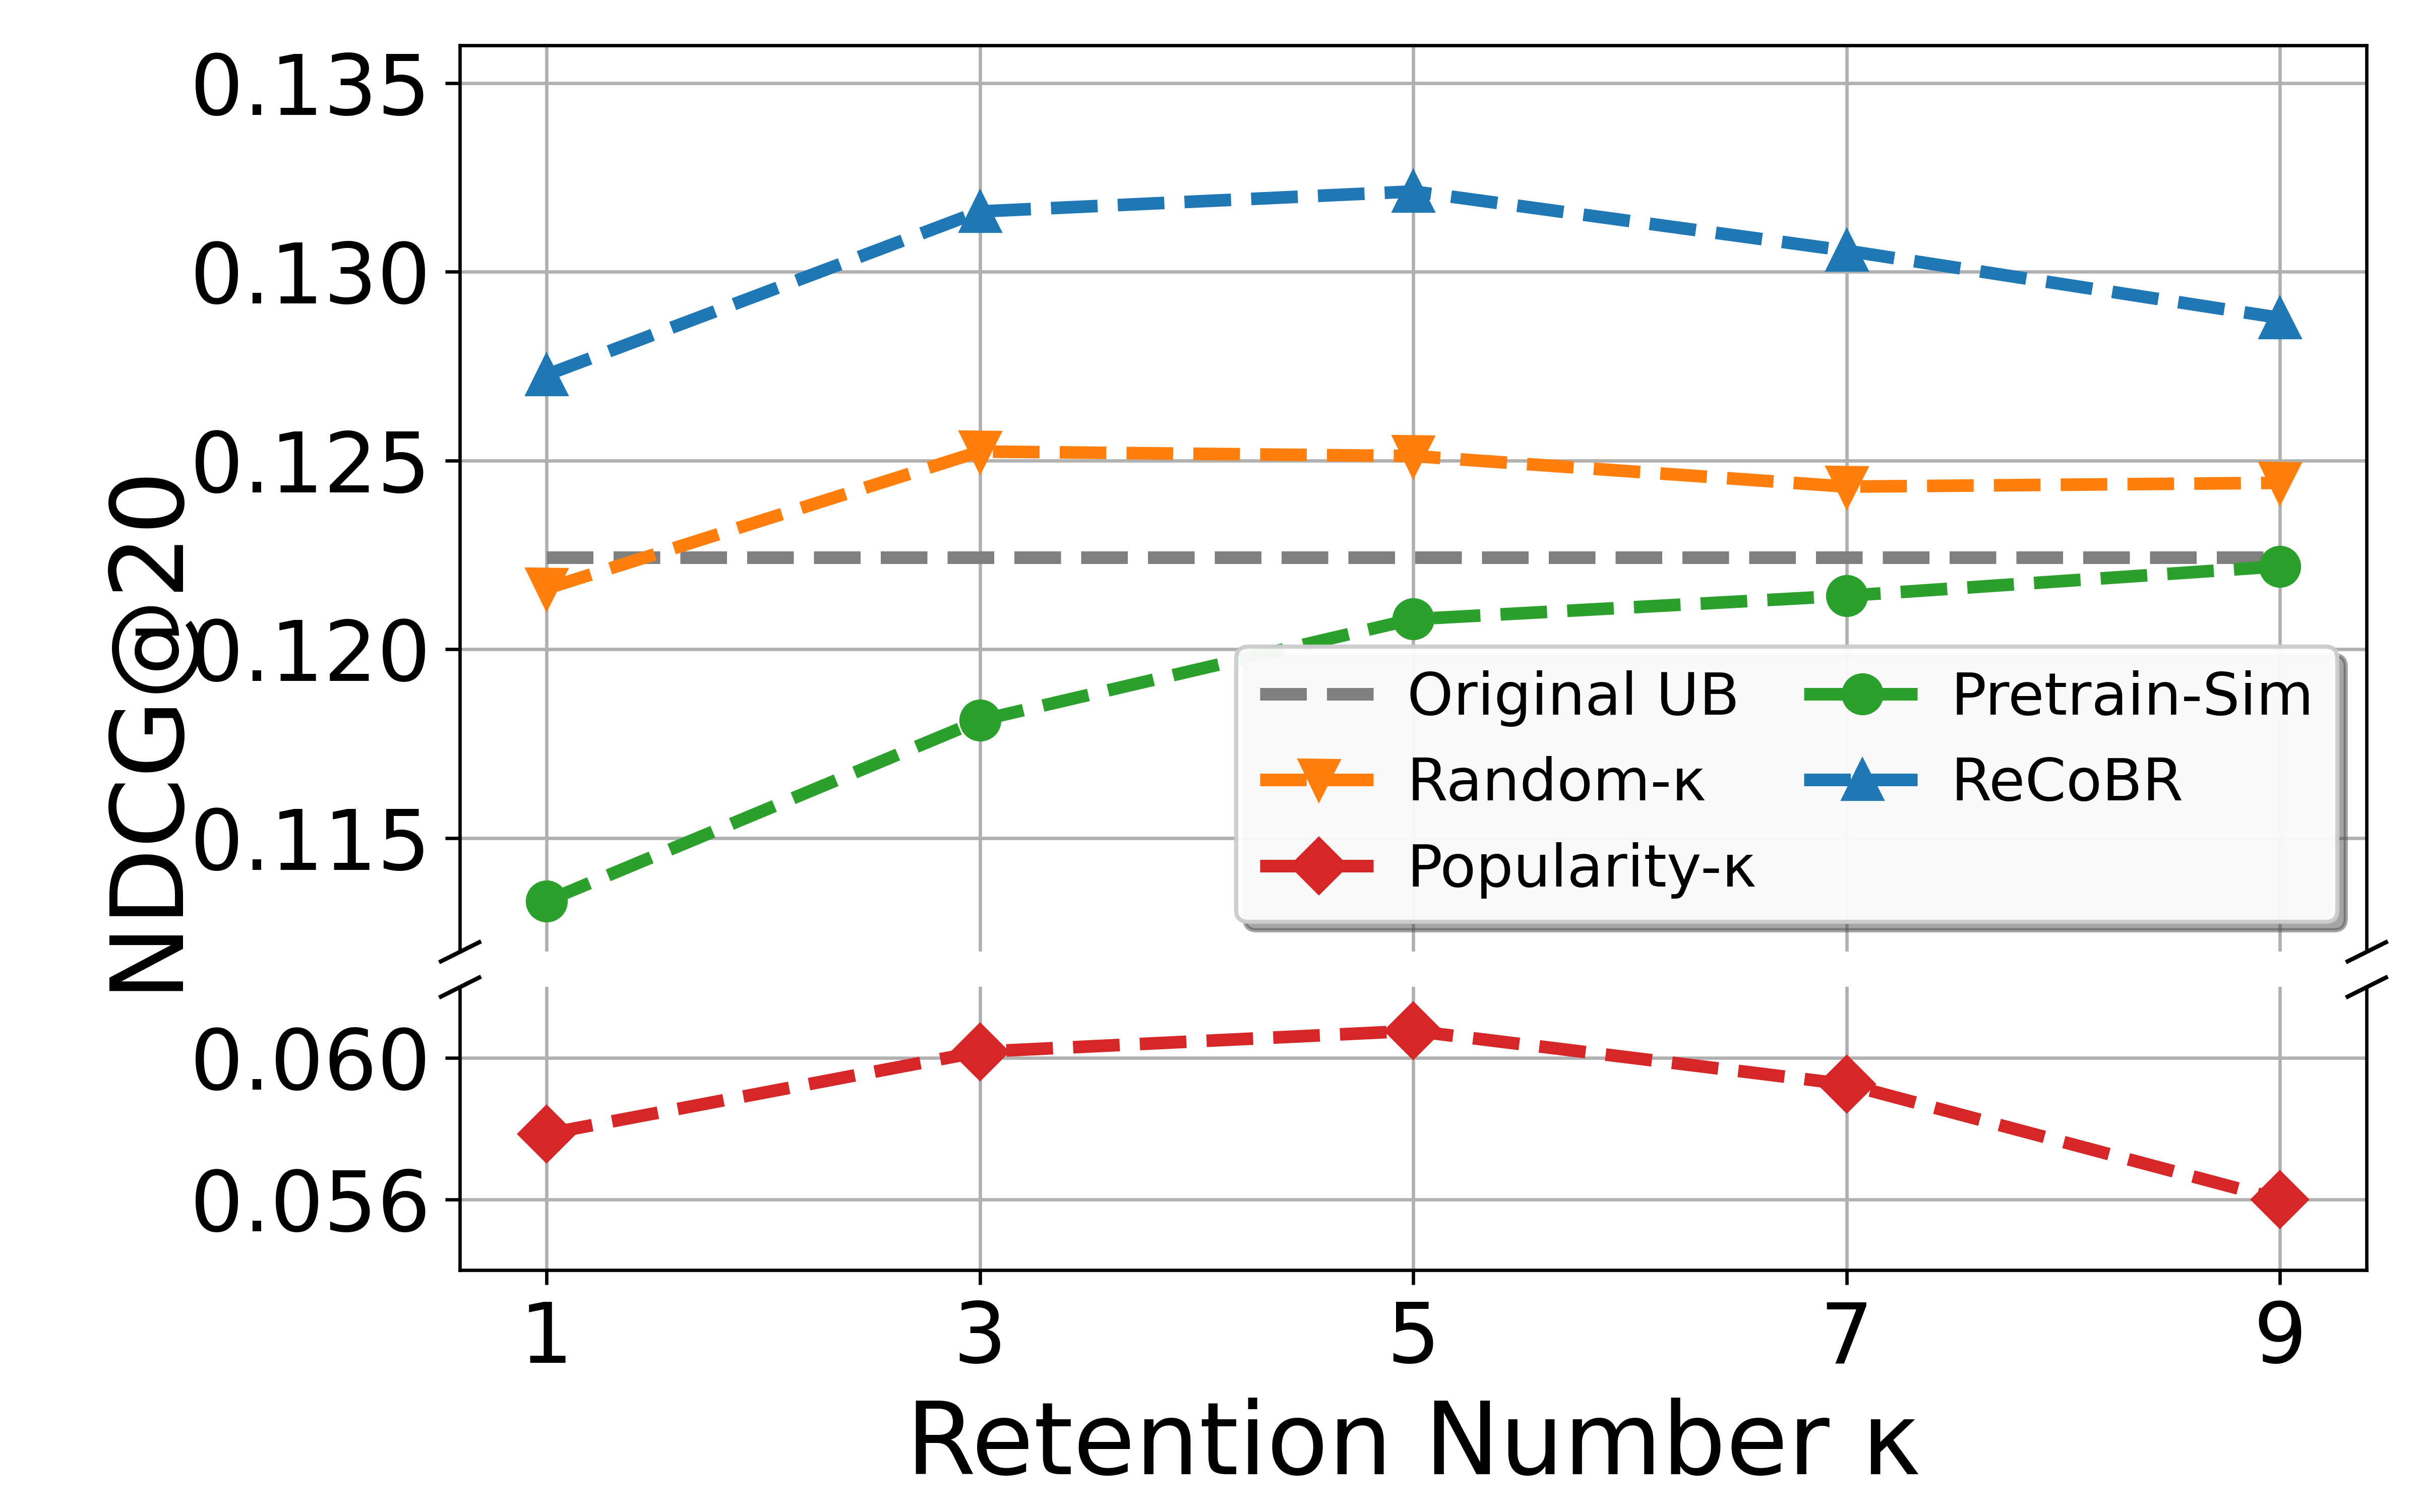
\includegraphics[width=0.46\columnwidth]
        {Figures/m1ndcg20.png} \\
        (a) & (b) \\
        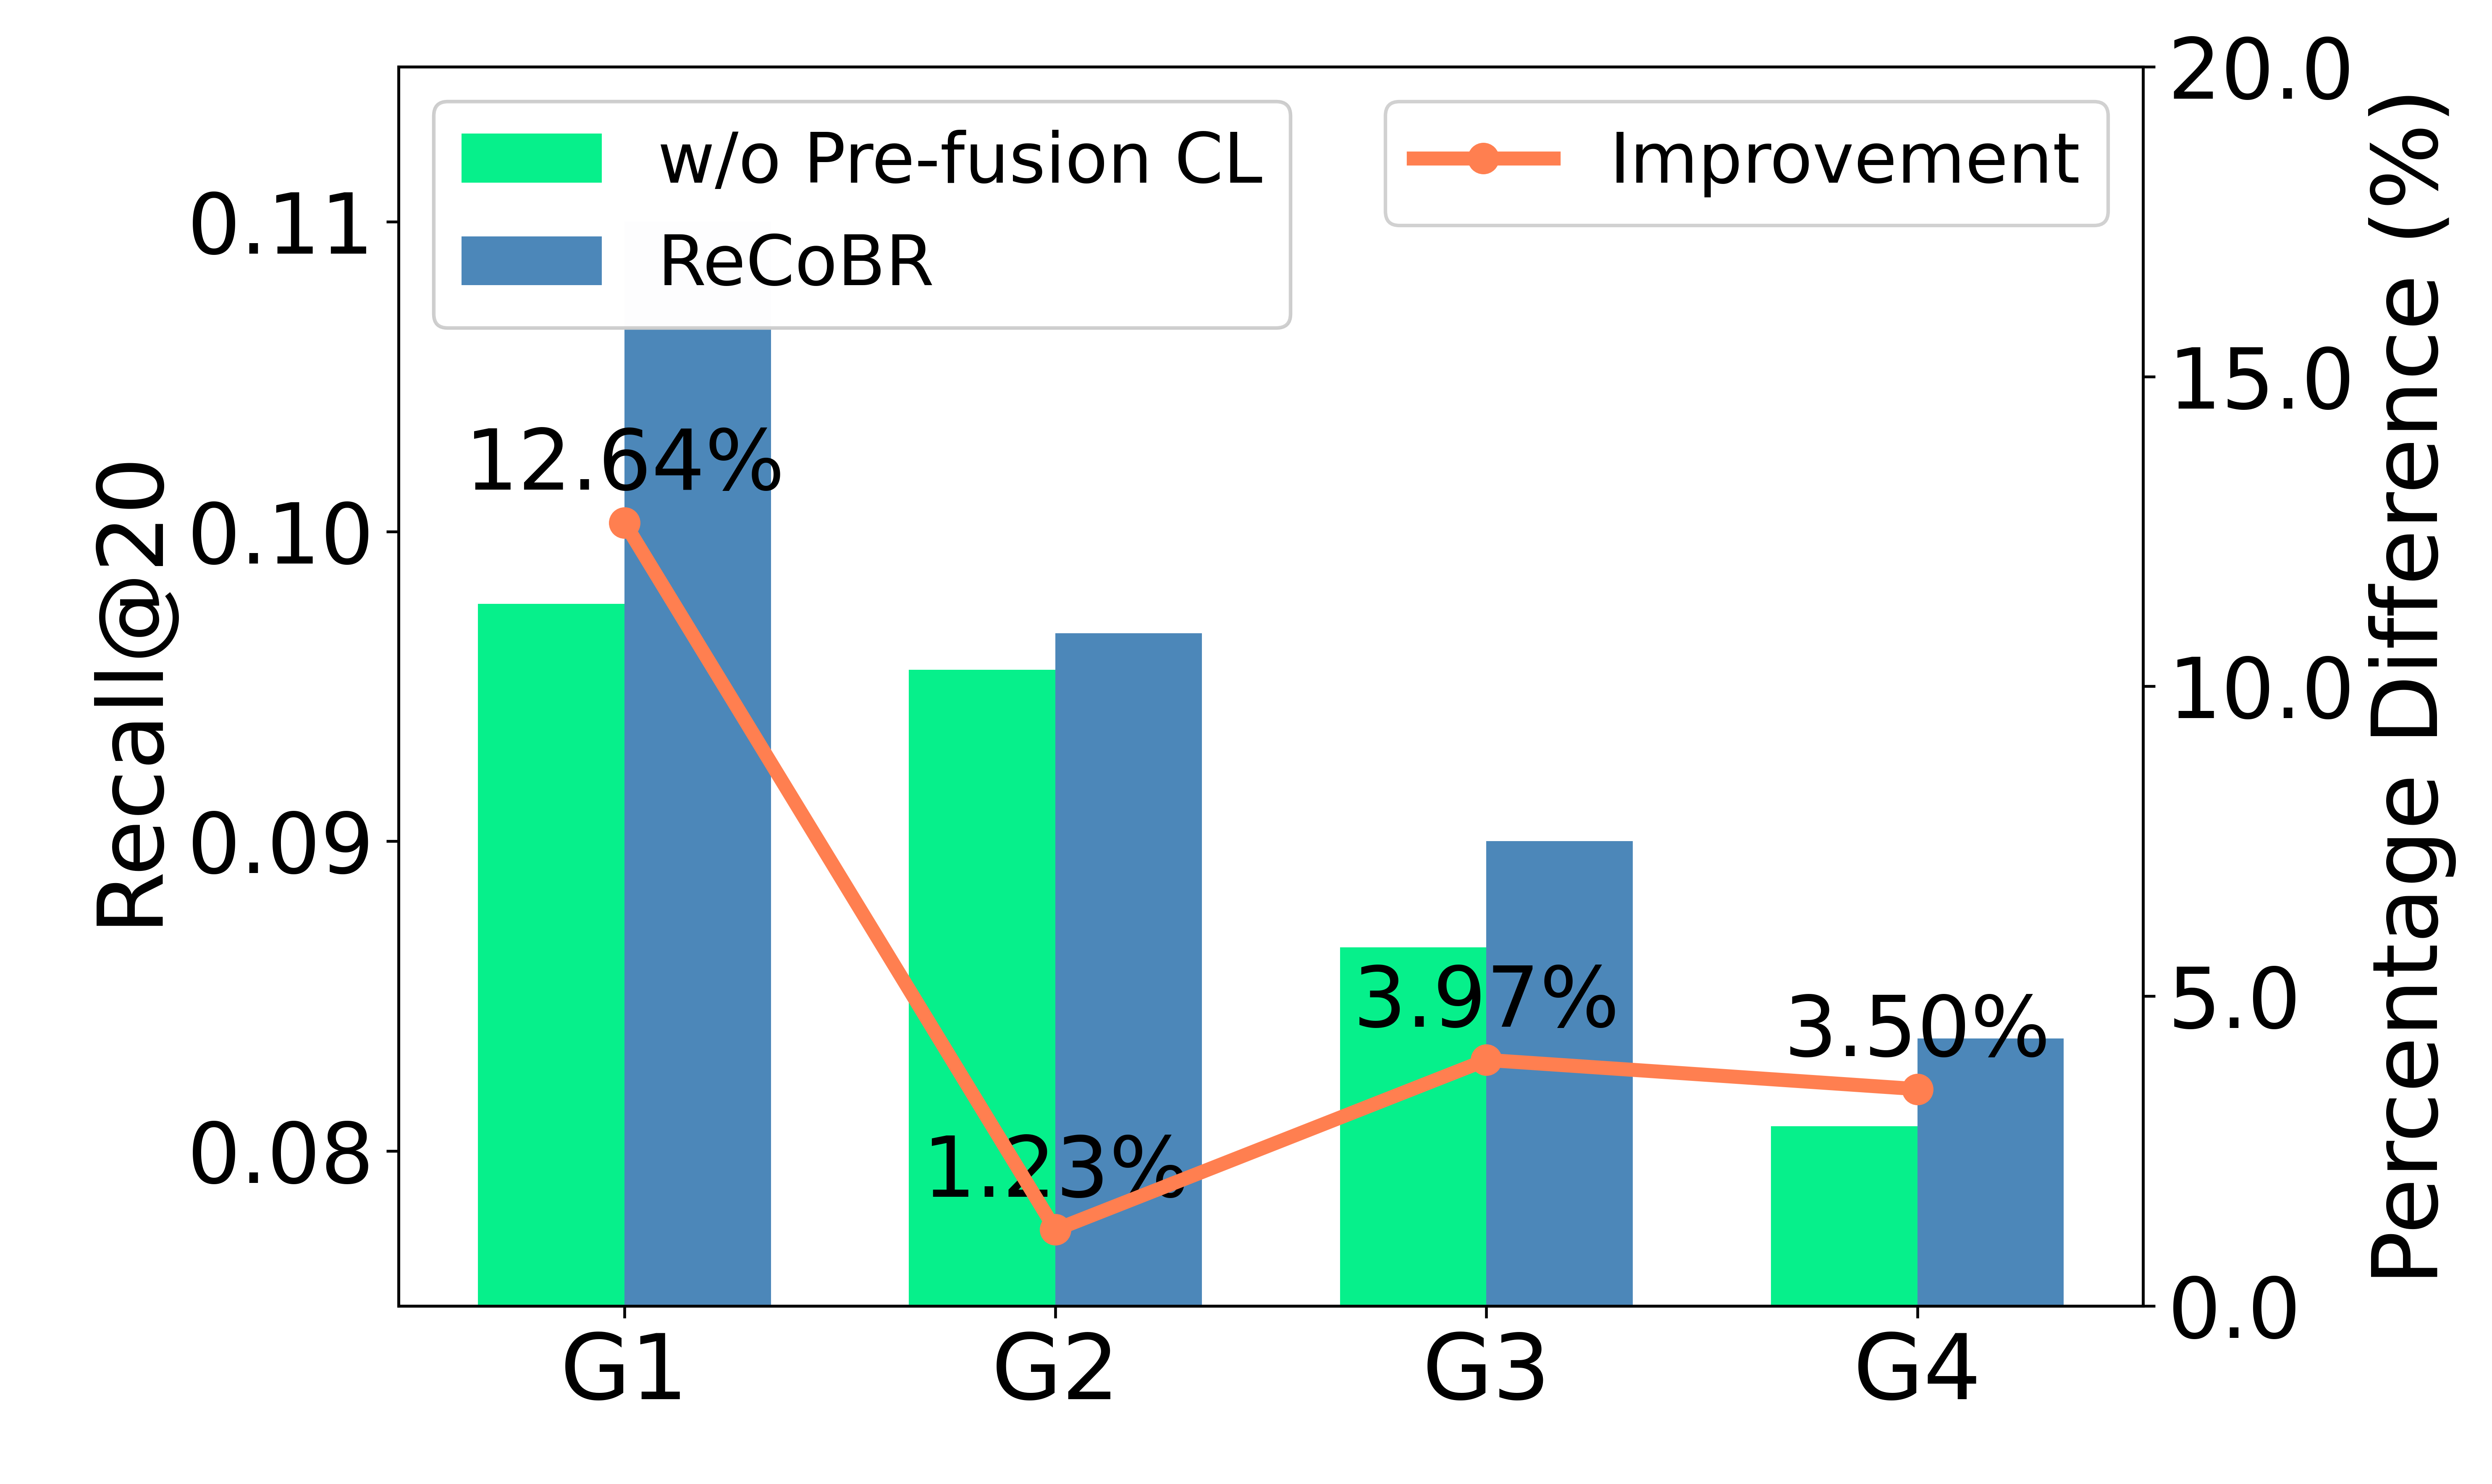
\includegraphics[width=0.46\columnwidth]
        {Figures/m2recall20.png} &
        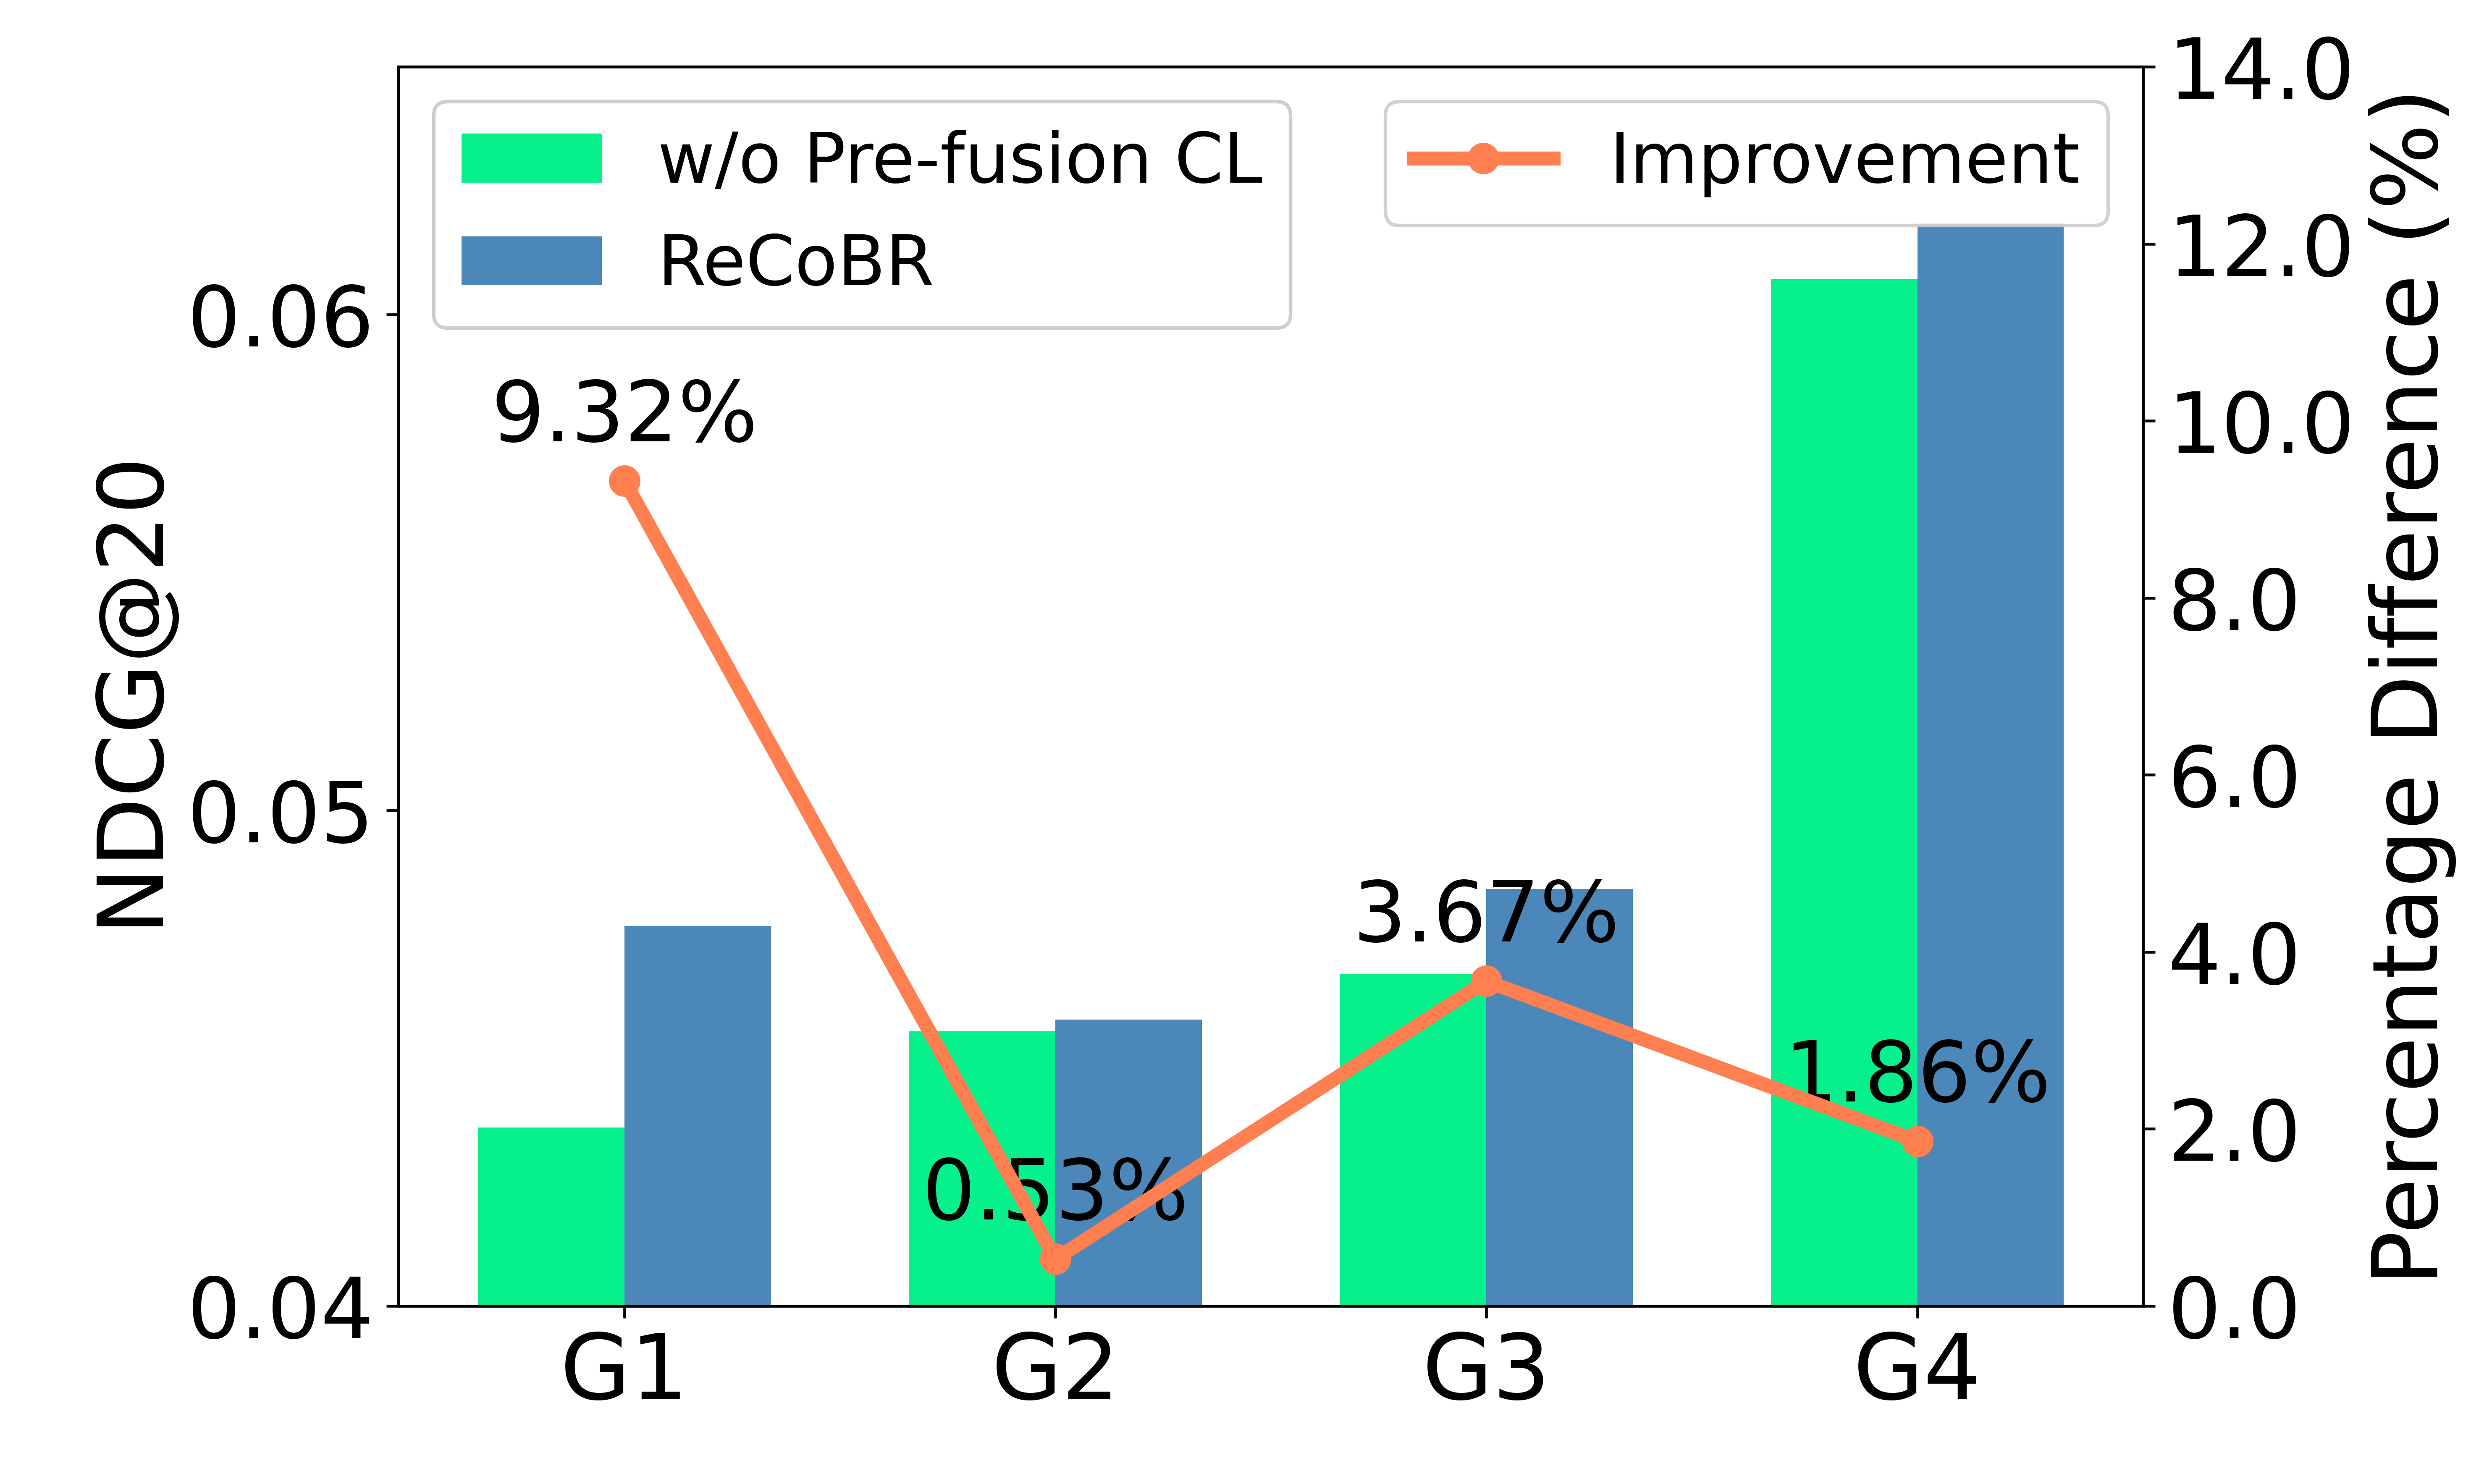
\includegraphics[width=0.46\columnwidth]
        {Figures/m2ndcg20.png} \\
        (c) & (d)
    \end{tabular}

    \caption{In-depth analysis of ReCoBR.
    (a)--(b) Recall@20 and NDCG@20 of interaction selection
    strategies on iFashion, with retention limit $\kappa$
    plotted as $K$.
    (c)--(d) Recall@20 and NDCG@20 of complete ReCoBR and
    w/o Pre-fusion CL on NetEase. Both retain graph
    reconstruction. G1--G4 are ordered by training U-B degree,
    with ranges $[0,7)$, $[7,8)$, $[8,12)$, and $[12,660]$.
    Lines show ReCoBR's relative gains over w/o Pre-fusion CL.}
    \label{fig:in-depth-analysis}
\end{figure}


\paragraph{Interaction Selection Strategies.}
To examine how the choice of retained interactions affects
recommendation, we compare five U-B graph construction
strategies on iFashion. \textbf{Original UB} keeps the observed
graph. \textbf{Random-$K$} retains randomly selected observed
interactions, whereas \textbf{Popularity-$K$} selects those
associated with the most popular bundles.
\textbf{Pretrain-Sim} scores interactions by the cosine
similarity of pretrained user and bundle embeddings.
\textbf{ReCoBR} instead scores them against the user's refined
historical bundle-preference vector. Each filtering strategy
retains at most $\kappa$ interactions per user, where $\kappa$
is denoted by $K$ in the figure, and selects only from the
user's training history. Results are averaged over multiple
independent runs.

Figure~\ref{fig:in-depth-analysis}(a)--(b) shows that ReCoBR
achieves the highest Recall@20 and NDCG@20 among the compared
strategies at every tested retention limit. Random selection
can improve over the original graph, but consistently trails
ReCoBR at matched retention limits. Thus, the choice of
connections matters beyond reducing their number.
Popularity-based selection is especially weak in NDCG,
indicating that globally popular bundles are not necessarily
the most useful propagation neighbors for an individual user.

Pretrain-Sim also underperforms ReCoBR. This comparison favors
the complete history-based refinement and scoring pipeline
over direct pretrained user--bundle similarity. ReCoBR's
performance initially improves as more interactions are
retained and then declines at larger limits. Together, these
observations support selecting connections according to
personalized bundle-preference context while balancing
neighborhood coverage and selectivity.


\begin{figure*}[t]
    \centering
    \begin{tabular}{@{}ccc@{}}
        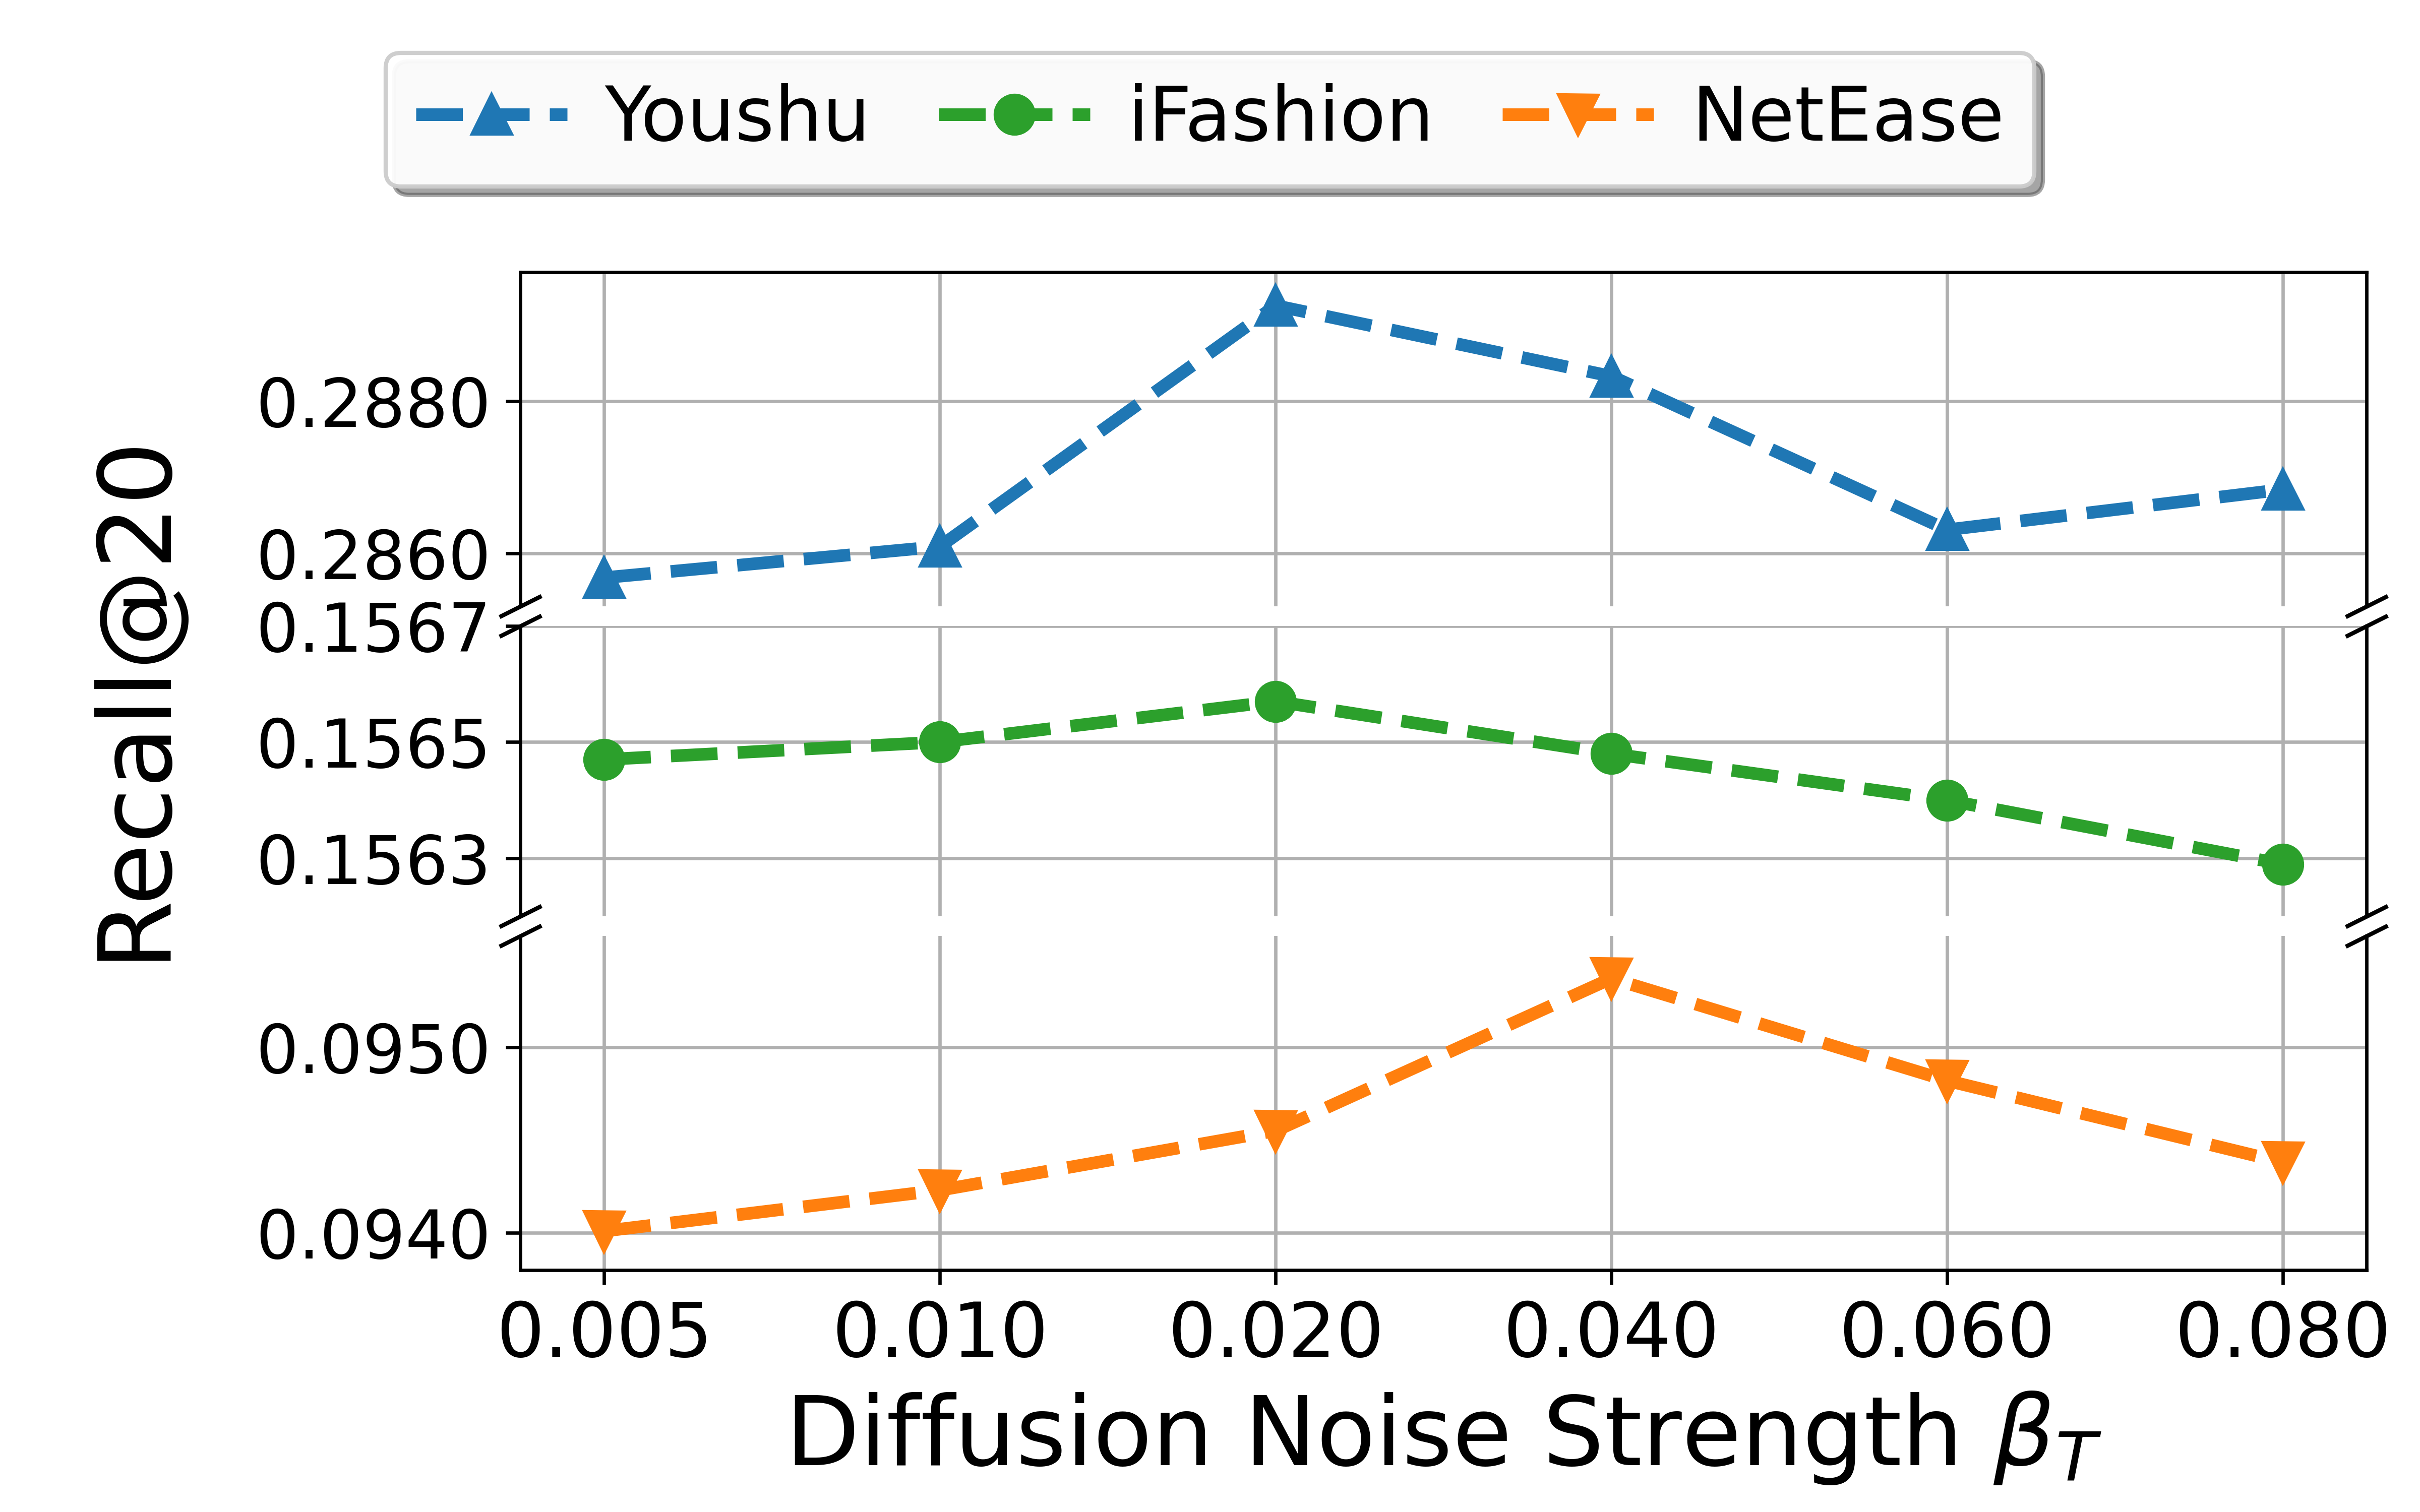
\includegraphics[width=0.31\textwidth]{Figures/hp_betaT.png} &
        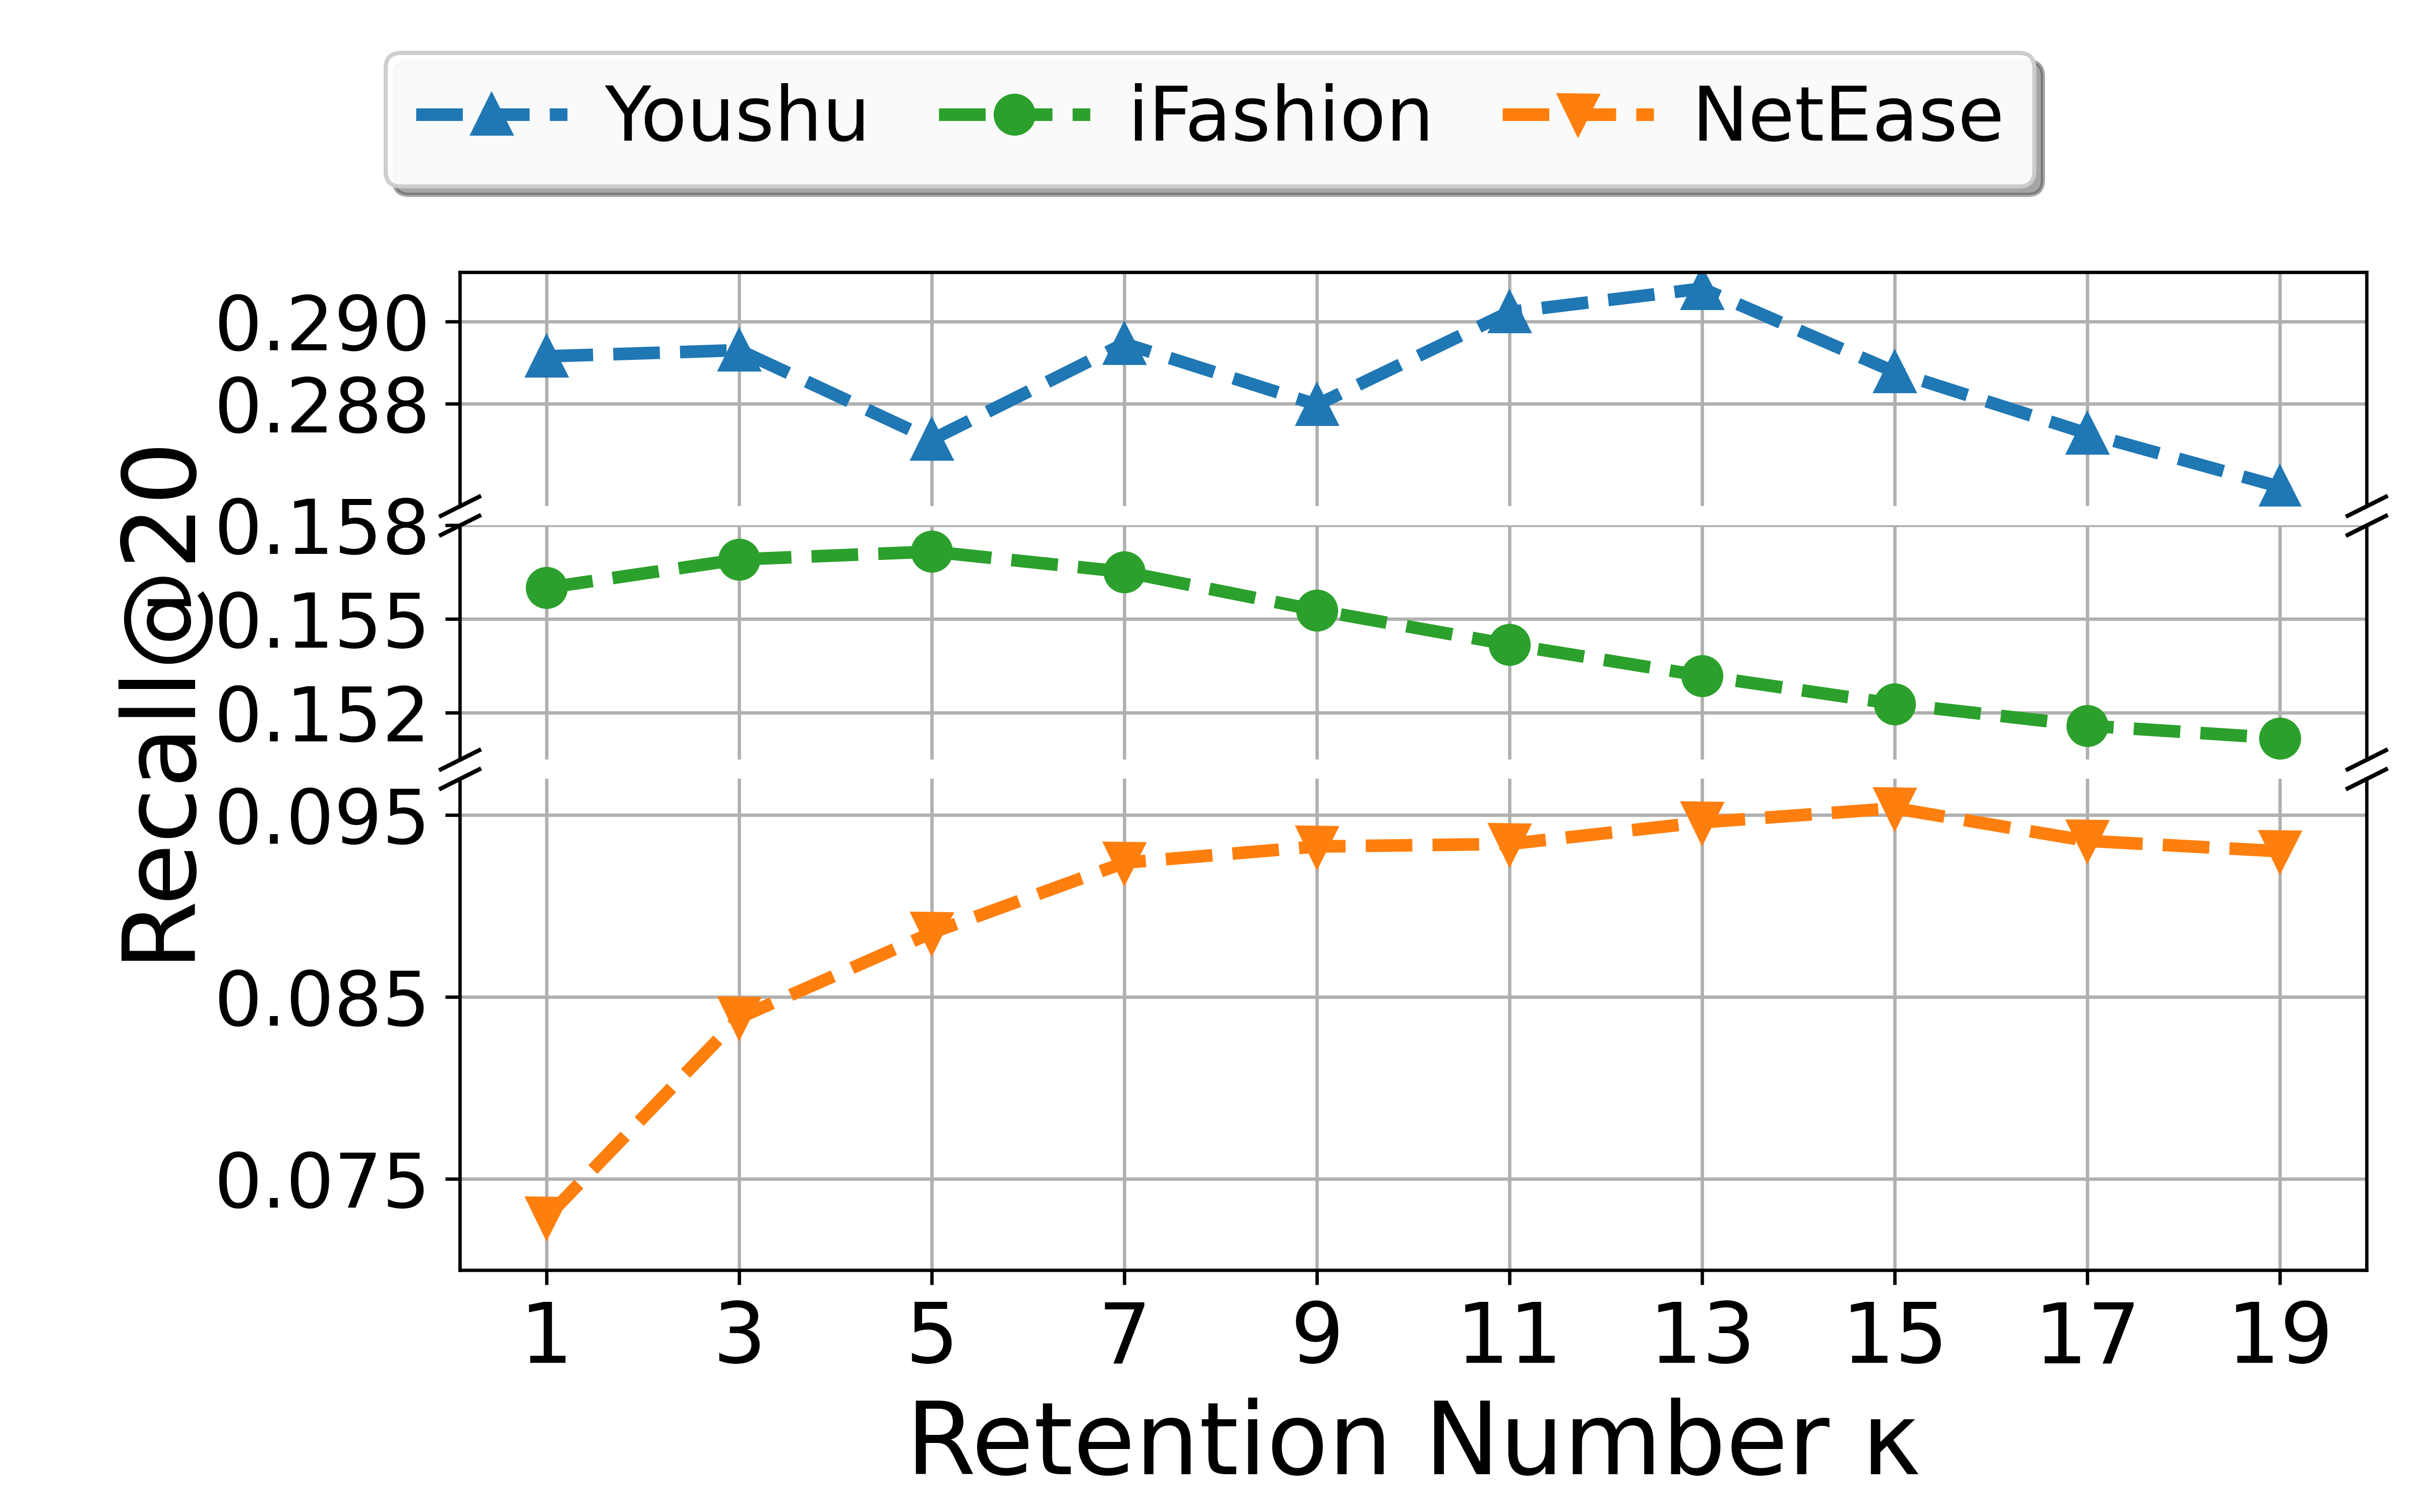
\includegraphics[width=0.31\textwidth]{Figures/hp_kappa.png} &
        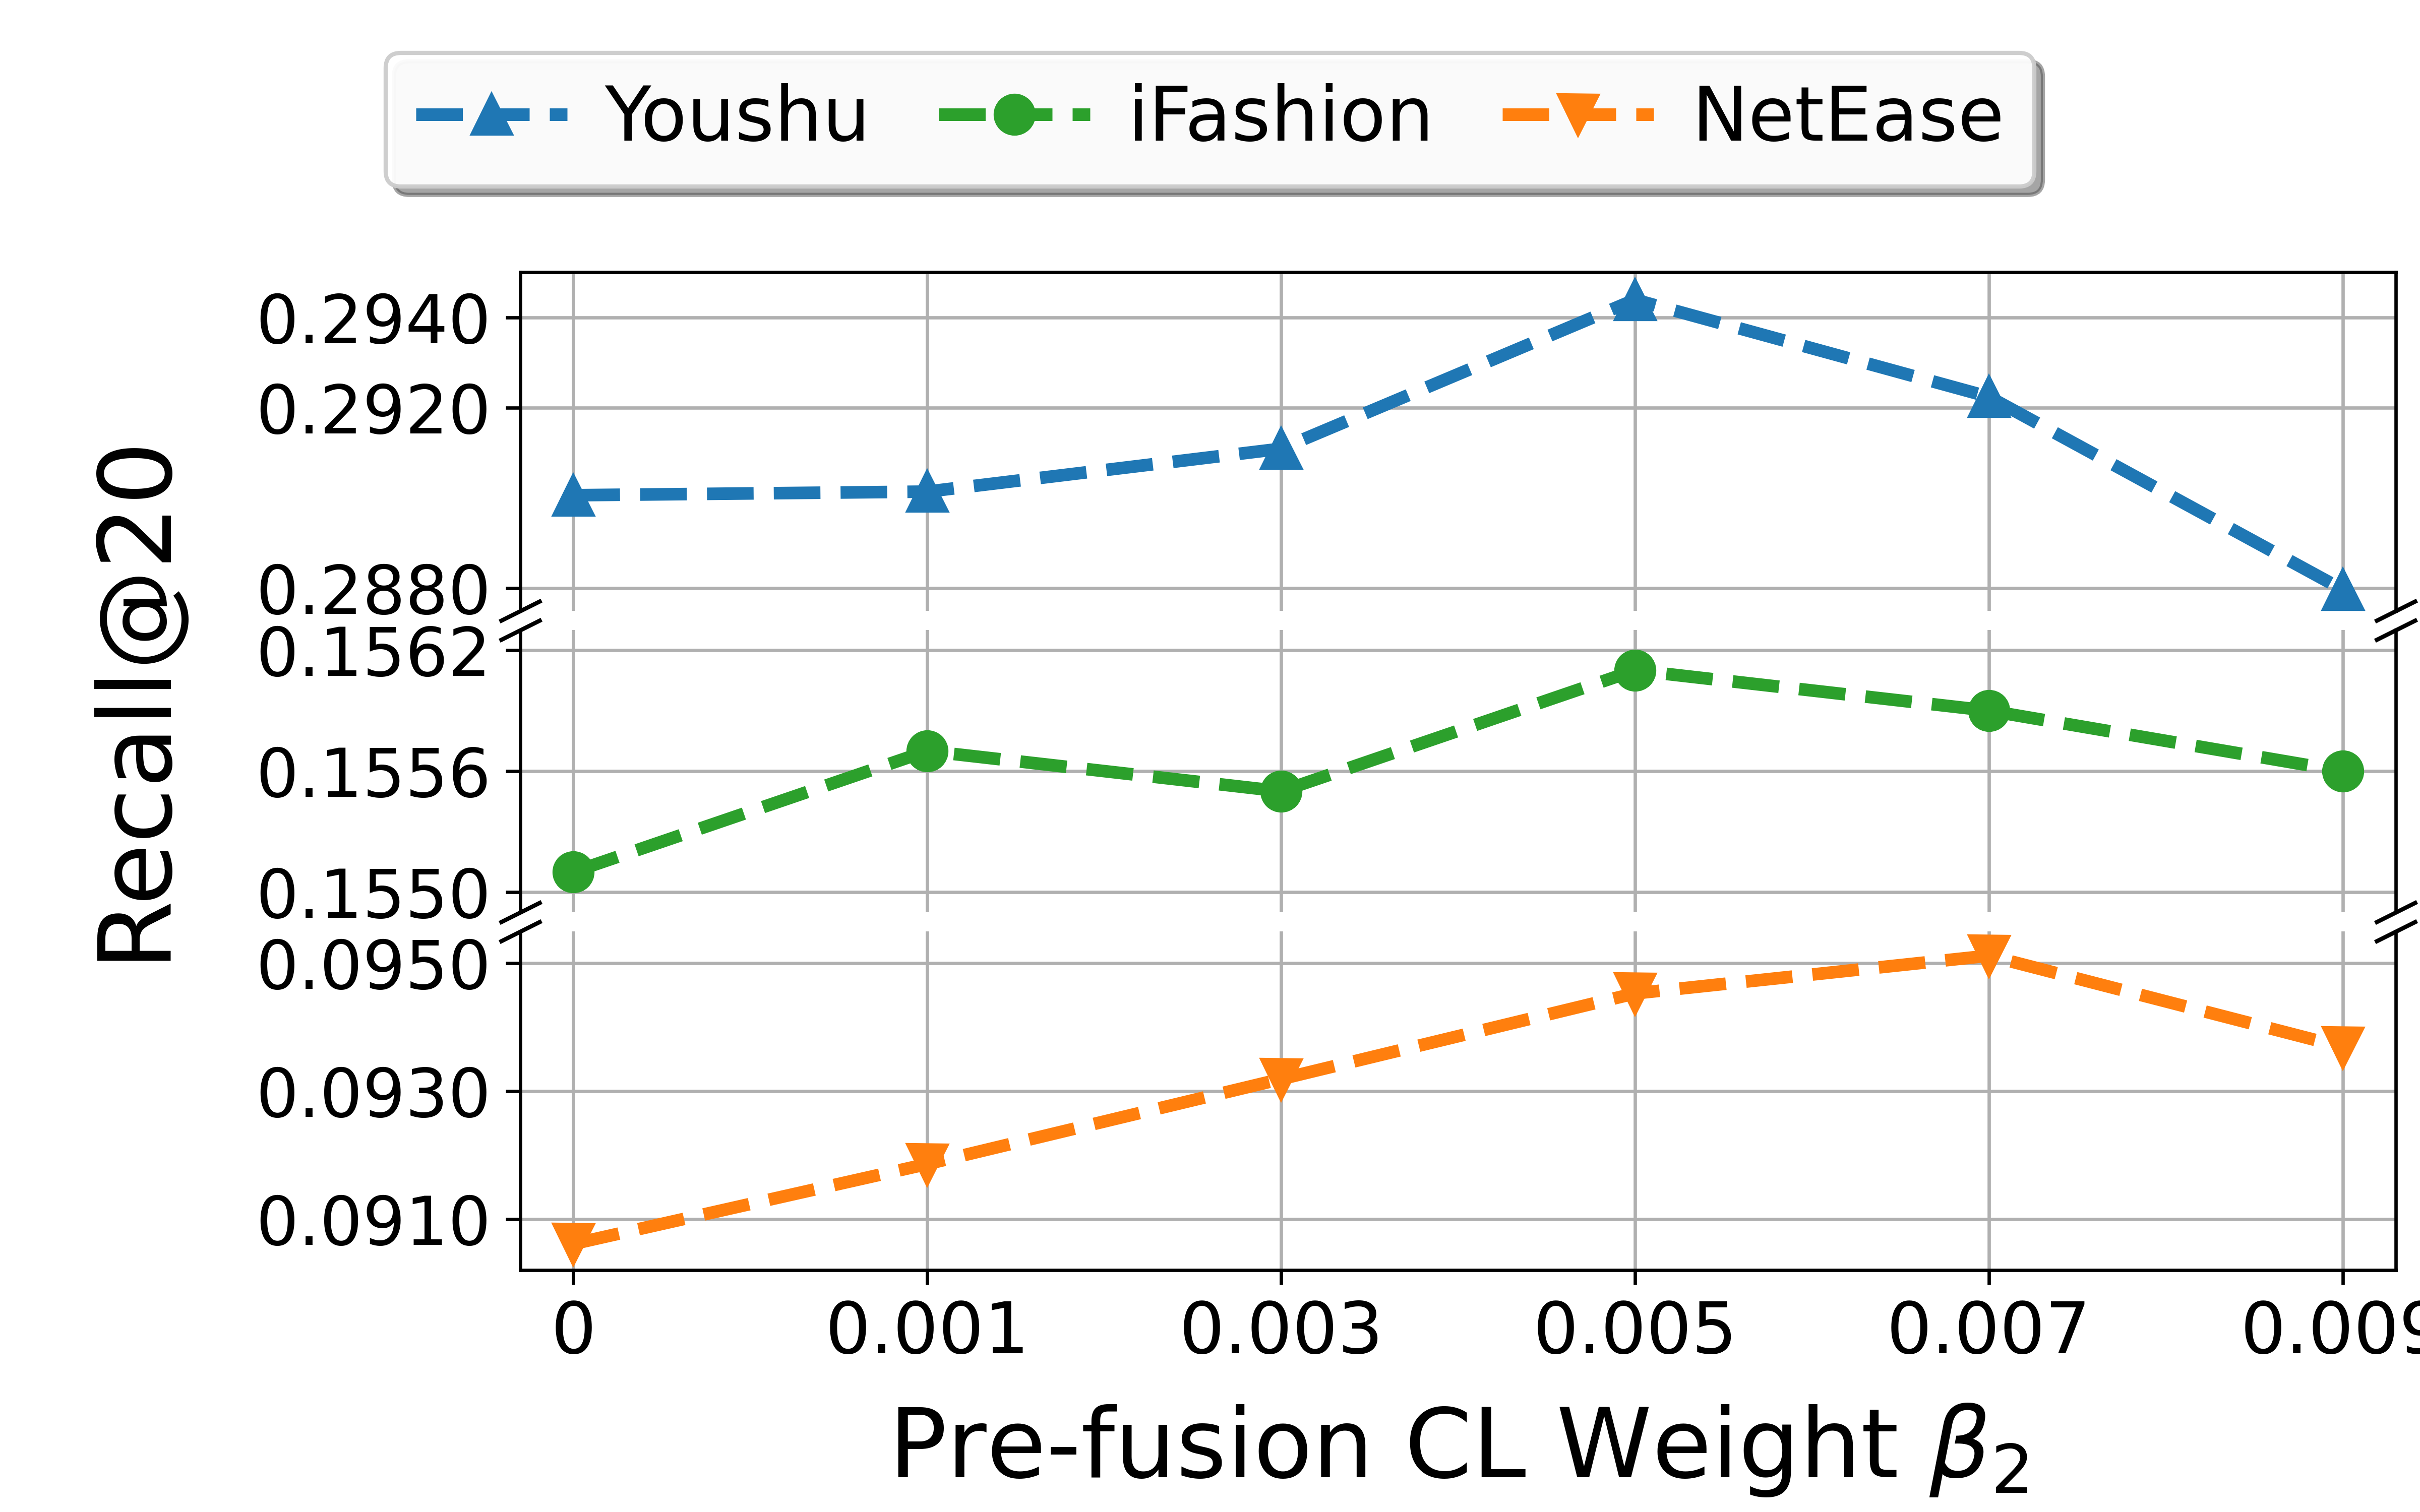
\includegraphics[width=0.31\textwidth]{Figures/hp_beta2.png} \\
        (a) & (b) & (c)
    \end{tabular}

    \caption{Hyperparameter sensitivity measured by Recall@20
    on three datasets. (a) Maximum per-step noise variance
    $\beta_T$ in the linear diffusion schedule.
    (b) Retention limit $\kappa$ for U-B graph reconstruction.
    (c) Pre-fusion contrastive weight $\lambda_a$, labeled
    $\beta_2$ in the plot. Broken $y$-axes separate the
    performance scales of the three datasets.}
    \label{fig:hyperparameter}
\end{figure*}


\paragraph{Performance on Sparse Users.}
To evaluate the pre-fusion objective under limited bundle
feedback, we group NetEase users by their numbers of training
U-B interactions, from the lowest-degree group G1 to the
highest-degree group G4. The degree ranges are given in
Figure~\ref{fig:in-depth-analysis}. We compare complete ReCoBR
with \textbf{w/o Pre-fusion CL}. Both settings retain
diffusion-driven graph reconstruction and the recommendation
backbone; they differ in whether the U-B-anchored cross-view
objective is included.

As shown in Figure~\ref{fig:in-depth-analysis}(c)--(d), ReCoBR
improves Recall@20 and NDCG@20 in all four groups. The largest
relative gains occur in G1: 12.64\% in Recall@20 and 9.32\%
in NDCG@20. Gains in the other groups are smaller and do not
decrease monotonically with interaction count. This result
directly supports the role of pre-fusion cross-view learning
under sparse U-B feedback. By associating U-B representations
with representations derived from U-I behavior and B-I
composition, the objective provides additional learning
signals for users with limited bundle histories. The gains
for G2--G4 further indicate that its benefit is not restricted
to the lowest-interaction users.


\subsection{Hyperparameter Sensitivity}

We vary the maximum diffusion noise variance $\beta_T$, the
retention limit $\kappa$, and the pre-fusion contrastive weight
$\lambda_a$ one at a time while keeping the other settings
fixed. Figure~\ref{fig:hyperparameter} reports Recall@20.

\paragraph{Diffusion Noise.}
Figure~\ref{fig:hyperparameter}(a) shows that intermediate
noise levels perform better than the ends of the tested range.
Youshu and NetEase exhibit clearer changes, whereas iFashion
varies within a narrower absolute range. Increasing $\beta_T$
makes the recovery task harder by perturbing the historical
preference more strongly. The observed curves are consistent
with balancing this training perturbation against preservation
of personalized information; stronger corruption does not
consistently improve recommendation.

\paragraph{Retention Limit.}
Figure~\ref{fig:hyperparameter}(b) reveals different responses
to $\kappa$. NetEase benefits markedly from increasing a very
small retained neighborhood, then levels off and slightly
declines. iFashion favors smaller limits and loses accuracy
as more connections are included. Youshu fluctuates within a
narrower range. These differences show that aggressive
filtering can discard useful propagation connections, while
retaining more observed edges is not always beneficial.
The retention limit should therefore account for the
dataset's balance between neighborhood coverage and
preference relevance.

\paragraph{Pre-Fusion Contrastive Weight.}
In Figure~\ref{fig:hyperparameter}(c), moderate nonzero weights
improve over omitting the cross-view objective, especially
on NetEase. Larger weights eventually reduce performance;
on Youshu, the largest tested weight also underperforms
zero weight. This behavior highlights the need to balance
cross-view agreement with the ranking objective, rather than
maximizing alignment strength. The scale of these changes
differs across datasets, as indicated by the broken axes.


\section{Conclusion}

We presented ReCoBR for bundle recommendation with noisy and
sparse U-B feedback. Its central design connects pretraining,
user-conditioned latent diffusion, and interaction selection
to reconstruct the graph used for recommendation. Within this
pipeline, bundle-set consistency adapts preference recovery
to the historical bundles used for subsequent scoring.
Pre-fusion cross-view contrastive learning then connects
representations from the reconstructed U-B graph with the
U-I and B-I views on both the user and bundle sides.

Experiments on three public benchmarks show improvements over
the compared baselines. Component ablations and interaction
selection analyses support the graph reconstruction pipeline
and the additional cross-view objective. The user-group
analysis further shows that pre-fusion learning yields its
largest relative gains for users with the fewest bundle
interactions. Together, these findings support refining the
U-B propagation graph and using its representations to guide
auxiliary-view learning as a way to improve bundle
recommendation under noisy and limited feedback.

\bibliography{aaai2027}

\end{document}
